\section{Messergebnisse und Auswertung}
\subsection{Allgemeines}
\subsubsection{Fehler und Zählrate}
\label{subsub:errorsandcounts}
Die Anzahl $N$ der Messereignisse von einem Kanal des MCAs ist poissonverteilt. Daher gilt für den Fehler $s_N$:
\begin{equation}
\label{eq:poisson:error}
  s_N = \sqrt{N}
\end{equation} 
Die Fehler wurden nur in den Graphiken für die Fits gezeichnet, damit beurteilt werden kann, ob der durchgeführte Fit die Messwerte innerhalb
ihrer Fehler beschreibt. Bei den Übersichten von den Gesamtspektren sind die Fehler weggelassen worden, um einen besseren Überblick zu gewähren. \\[\baselineskip]
Aufgrund der unterschiedlichen Messzeiten wird die Anzahl $N$ der Messereignisse durch die verstrichene Zeit $t$\footnote{ohne Totzeit}
auf eine Zählrate $n$ normiert. Dementsprechend werden auch die Fehler $s_N$ angepasst.
\begin{equation}
\label{eq:countrate}
  n = \frac{N}{t}, \qquad s_n = \frac{s_N}{t}
\end{equation}

\subsubsection{Gauß-Verteilung}
\label{subsub:gaus}
Bei der Auswertung wird oft die Gauß-Verteilung als theoretisches Modell (also auch als Fit-Modell) der Messwerte verwendet. Es wird folgende 
Konvention\footnote{gemäß der Funktionenbenennung in ROOT} eingeführt:
\begin{equation}
  \label{eq:gaus}
  \gaus(x; A, c, s) = A \cdot e^{-\frac{1}{2} \left( \frac{x - c}{s} \right)^2}
\end{equation}
wobei $\gaus(x; A, c, s)$ eine Funktion von $x$ mit Parametern $A$ (Amplitude), $c$ (Erwartungswert\footnote{$c=$ channel}) und 
$s$ (Standardabweichung) ist.

\subsection{\textgamma-Spektrum des Untergrundes}
Das Untergrundspektrum ist in \autoref{img:underground:spectrum} abgebildet. Man erkennt einen Peak bei Kanal 3600, der aufgrund der noch 
fehlenden Energieeichung erst in \ref{sub:eval:undergroundpeak} diskutiert wird. Bei kleineren Kanälen (was einer kleineren Energie entspricht) ist 
die Zählrate tendenziell höher, was auf eine höhere Anzahl von niederenergetischer Strahlung zurückzuführen ist. 
\begin{figure}[H]
\begin{center}
  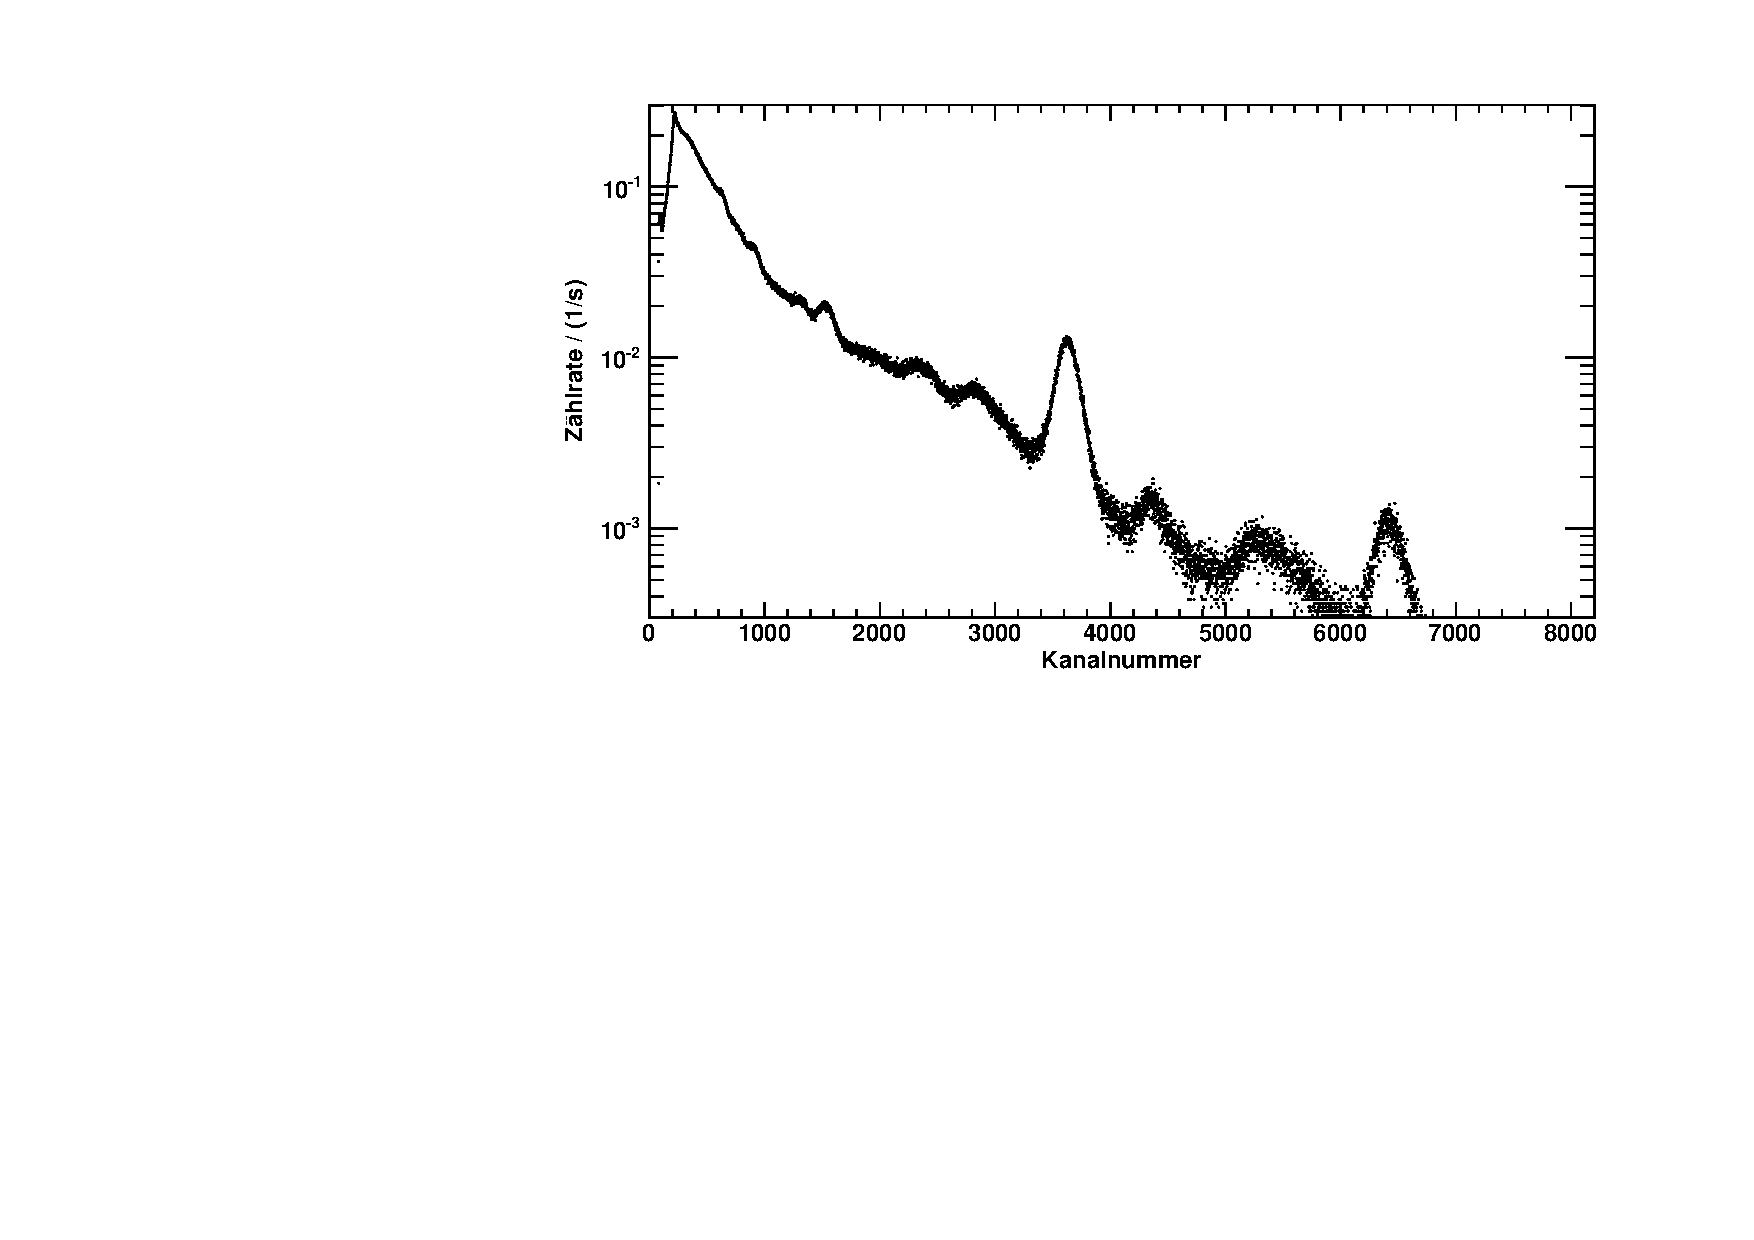
\includegraphics[width=\textwidth]{../img/underground_spectrum.pdf}
  \caption{\textgamma-Spektrum des Untergrundes}
  \label{img:underground:spectrum}
\end{center}
\end{figure}
Um eine gute Auswertung der Messungen zu erreichen, ist es notwendig den Untergrund $u$ von den gemessenen Werten $n'$ abzuziehen. Man erhält 
somit untergrundbereinigte Messwerte $n$. Der Fehler auf diese wird mit der Gauß'schen Fehlerfortpflanzung berechnet.
\begin{equation}
  n = n' - u, \qquad s_n = \sqrt{s_{n'}^2 + s_u^2}
\end{equation}
Im folgenden sind alle Spektren untergrundbereinigt.

\subsection{Energieeichung des Vielkanalanalysators}
Um eine Beziehung der Kanäle des Vielkanalanalysator(MCA) und der den Kanälen entsprechenden Energien herzustellen, wurden die Spektren von Elementen 
mit bekannten Energien von den Peaks gemessen. Diese Peaks werden nun analysiert um letztendlich eine Funktion für die Energie in Abhängigkeit des 
Kanals des MCAs zu finden.
\subsubsection{Peaks von \na}
\label{subsub:eval:na}
Das gesamte Spektrum von \na\,ist in \autoref{img:na:spectrum} dargestellt. Da sich die Probe von \na\, von den anderen unterscheidet, konnten nicht die 
gleichen Bedingungen wie bei der Untergrundmessung hergestellt werden. Der als Halterung und zur Abschirmung verwendete Bleiblock konnte nicht 
benutzt werden. Deshalb ist trotz Bereinigung des Untergrundes noch ein Untergrund zu sehen. Vor allem die ansonsten vom Bleiblock abgeschirmte 
niederenergetische Strahlung sticht dabei besonders hervor. Außerdem gibt es aus dem gleichen Grund auch einige negative Zählraten, welche jedoch 
außerhalb von den für uns relevanten Bereichen liegen.
\begin{figure}[H]
\begin{center}
  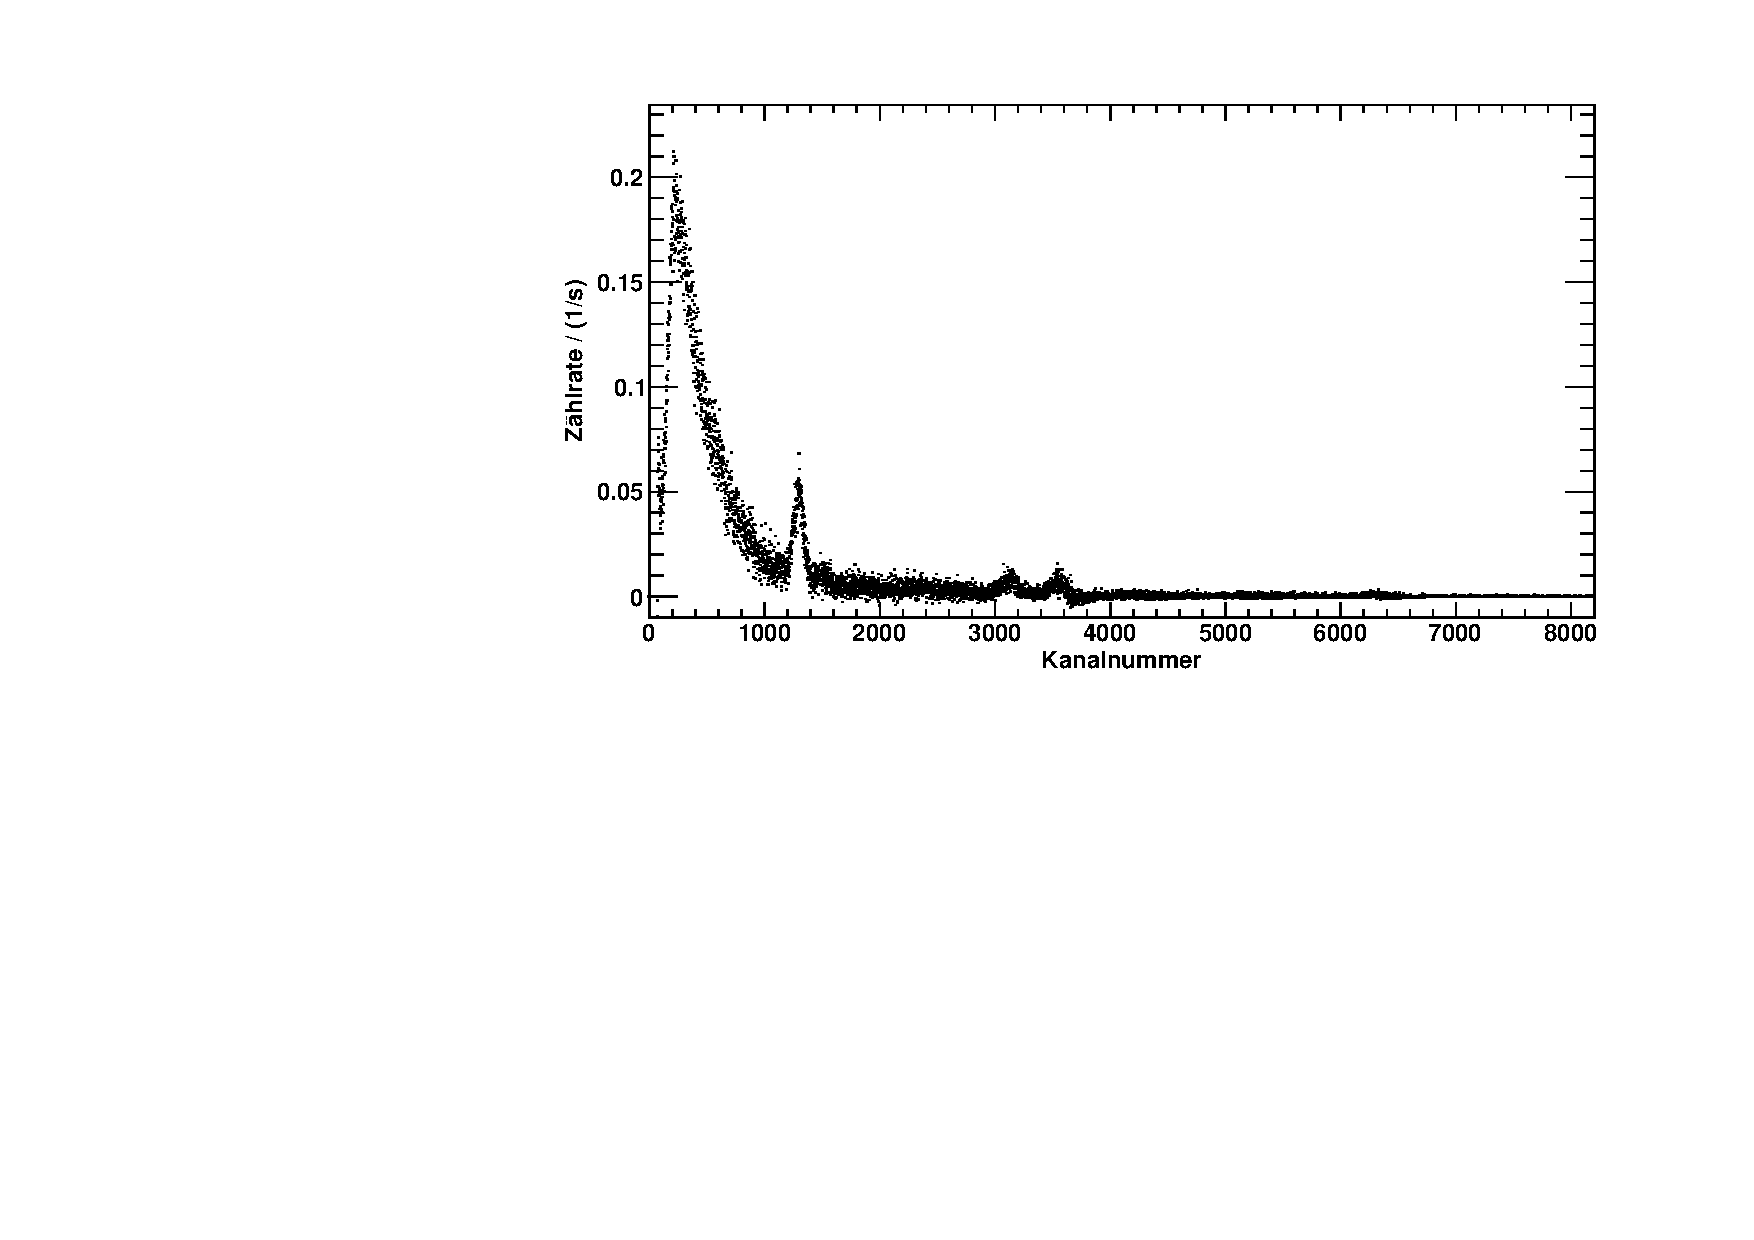
\includegraphics[width=\textwidth]{../img/na_spectrum.pdf}
  \caption{\textgamma-Spektrum von \chemel{Na}{22}}
  \label{img:na:spectrum}
\end{center}
\end{figure}
Trotz des nichtverschwindenden Untergrundes lässt sich der 511\,keV-PEak gut erkennen. Des weiteren sind zwei weitere Peaks mit geringerer 
Zählrate bei Kanal 3100 und 3500 zu erkennen. Ein Vergleich mit dem Spektrum des Untergrundes \autoref{img:underground:spectrum} identifiziert 
den zweiten Peak als Folge des Untergrundes (und nicht vollständiger Abschirmung dessen). Damit kann der erste Peak \na\,zugeordnet werden.\\[\baselineskip]
Die beiden Peaks von \na\, werden nun jeweils mit einer Gauß-Verteilung (Kapitel \ref{subsub:gaus}), verziert mit einem linearen Untergrund, 
gefittet, um den genauen Kanal des Maximums zu bestimmen:
\begin{equation}
  y_i = a_i + b_i \cdot x + \gaus(x; A_i, c_i, s_i), \qquad i = 1, 2
\end{equation}
Der Fit ist in \autoref{img:na:peaks} zu sehen. Man erhält folgende Werte für die Kanäle:
\begin{equation}
\begin{split}
  \label{eq:na:channels}
  c_1 &= 1302.4  \pm 1.7 \\
  c_2 &= 3135  \pm 5 
\end{split}
\end{equation}
\begin{figure}[H]
\begin{center}
  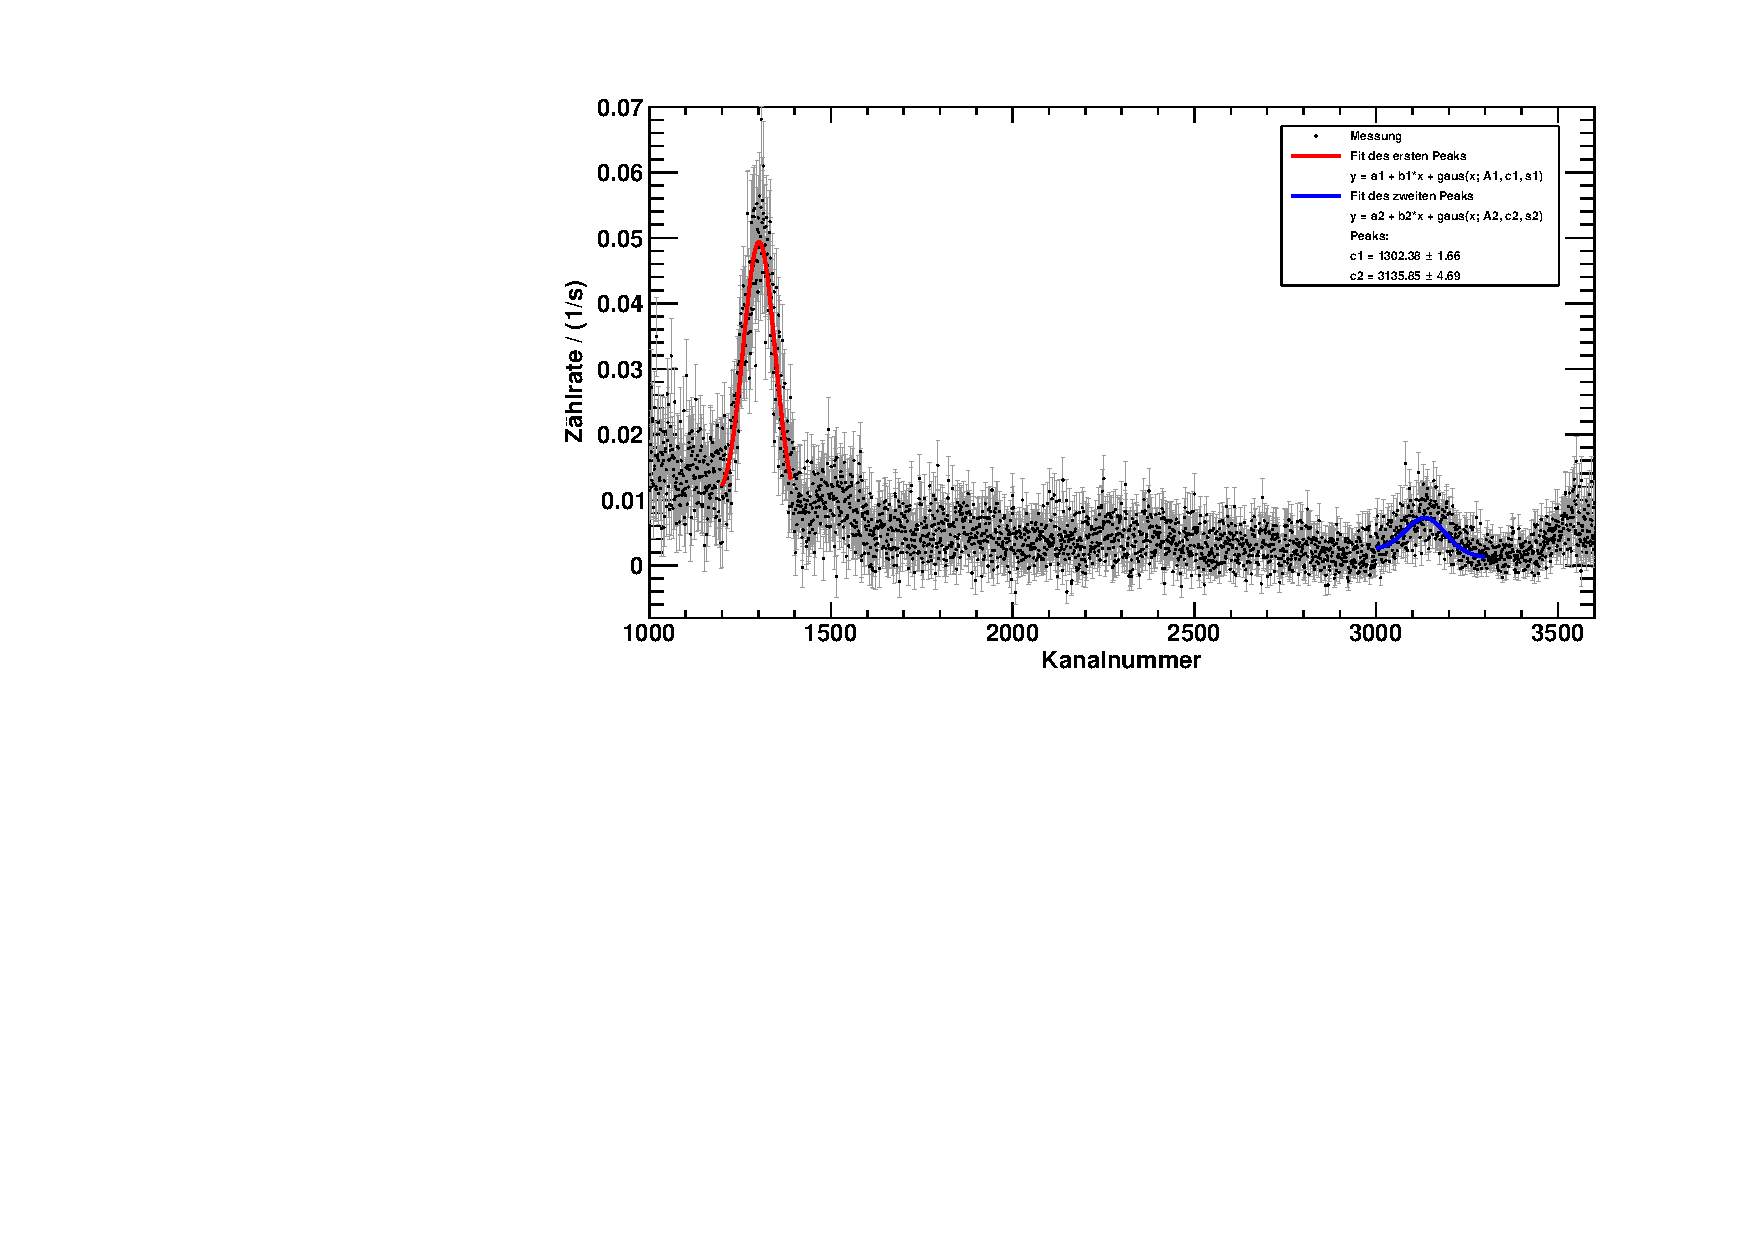
\includegraphics[width=\textwidth]{../img/na_peaks.pdf}
  \caption{Fit der beiden Peaks (511\,keV und 1274\,keV) von \na\, mit jeweils einem linearen Untergrund und einer Gauß-Verteilung.}
  \label{img:na:peaks}
\end{center}
\end{figure}

\subsubsection{Peaks von \co}
\label{subsub:eval:co}
In \autoref{img:co:spectrum} ist das Spektrum von \co abgebildet. Man erkennt gut den Doppelpeak zwischen den Kanälen 2800 und 3400.
\begin{figure}[H]
\begin{center}
  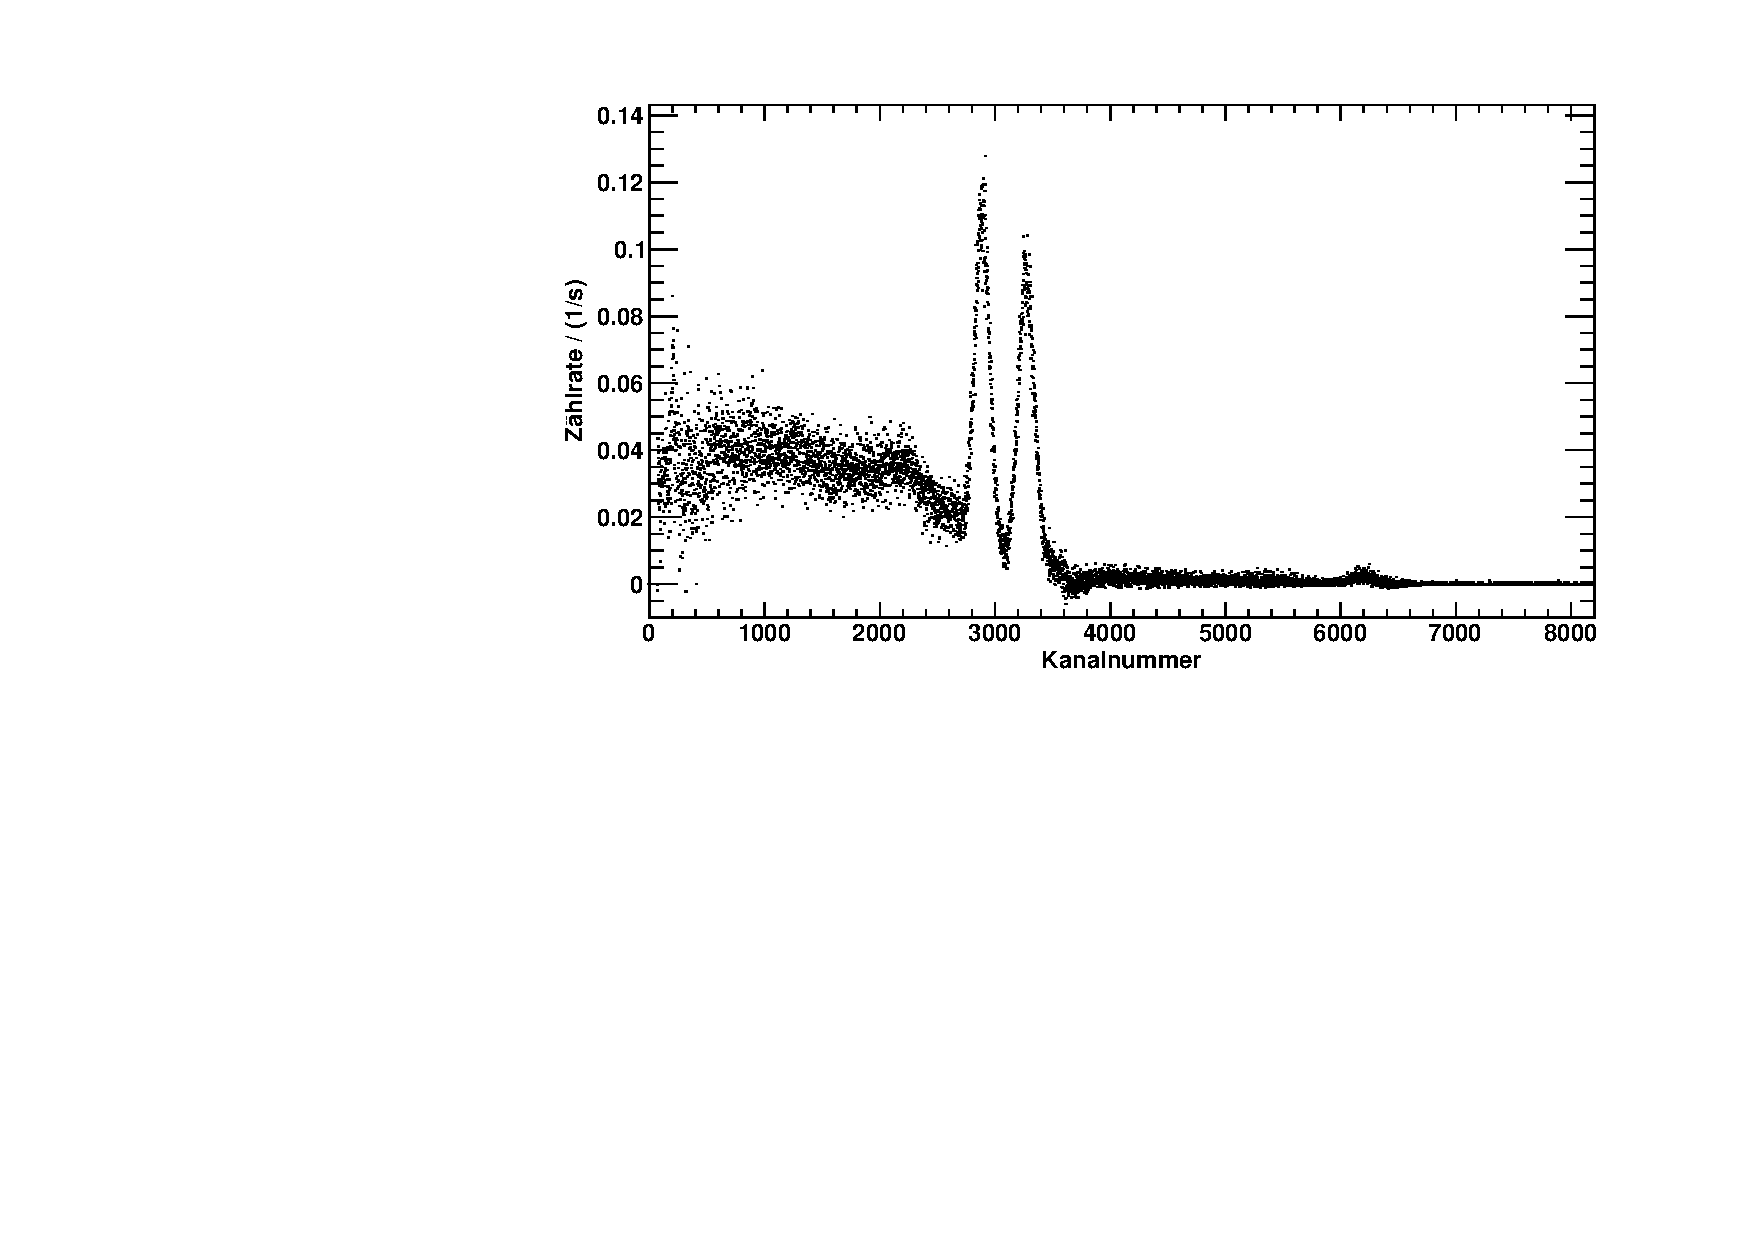
\includegraphics[width=\textwidth]{../img/co_spectrum.pdf}
  \caption{\textgamma-Spektrum von \chemel{Co}{60}}
  \label{img:co:spectrum}
\end{center}
\end{figure}
Die beiden Peaks wurden mit folgender Funktion gefittet:
\begin{equation}
  y = a + b\cdot x + \gaus(x; A_1, c_1, s_1) + \gaus(x; A_2, c_2, s_2)
\end{equation}
Es wurde wieder ein linearer Untergrund angesetzt, jedoch wurden diesmal im Gegensatz zu den Peaks von \na\, beide Peaks gleichzeitig gefittet. 
Dies wird mit der Nähe der beiden Peaks zueinander begründet, da sie sich womöglich überlappen und somit gegenseitig ihre Form beeinflussen.\\
Der Fit ist in \autoref{img:co:peaks} angezeigt und liefert folgende Werte:
\begin{equation}
\begin{split}
  \label{eq:co:channels}
  c_1 &= 2897.3 \pm 0.5 \\
  c_2 &= 3283.3 \pm 0.6
\end{split}
\end{equation}
\begin{figure}[H]
\begin{center}
  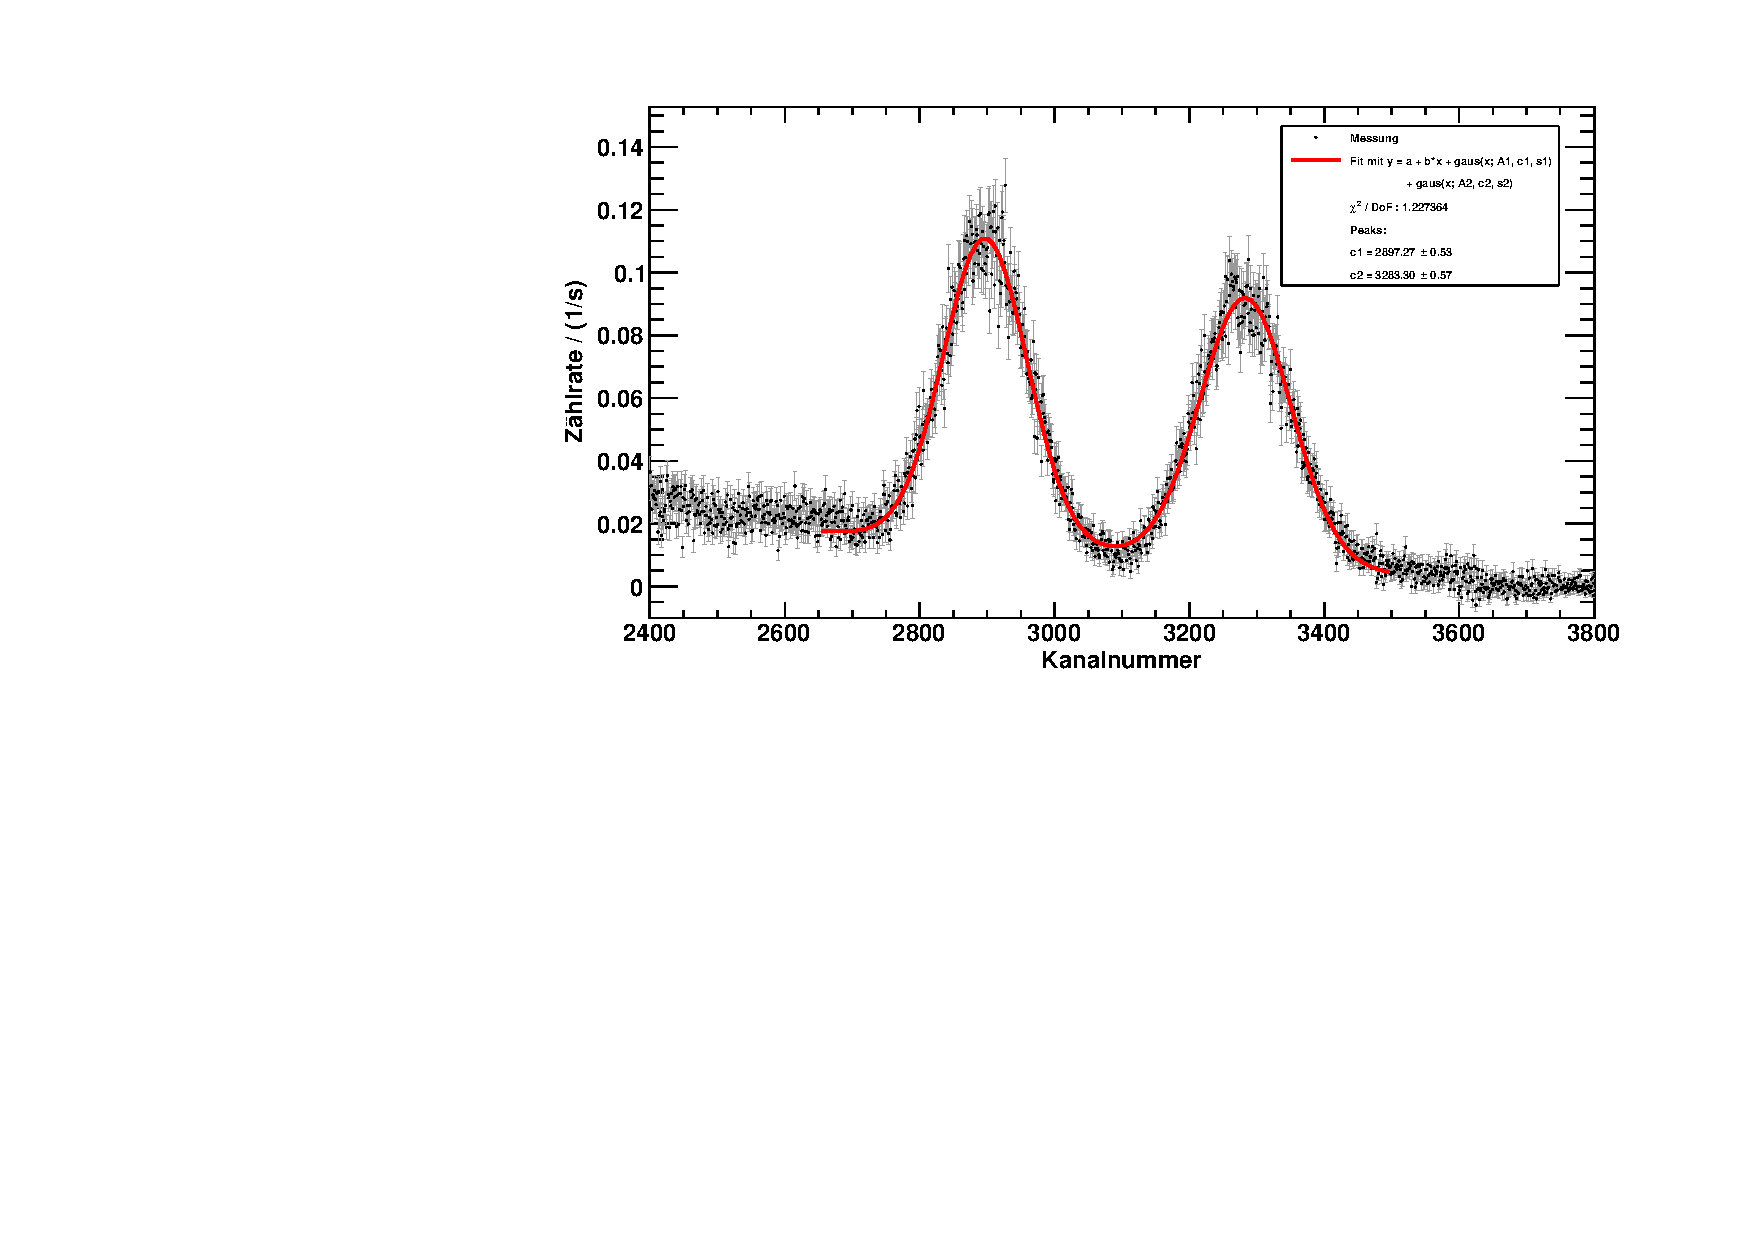
\includegraphics[width=\textwidth]{../img/co_peaks.pdf}
  \caption{Fit der beiden Peaks (1172\,keV und 1332\,keV) von \co\, mit einem linearen Untergrund und sich zwei überlagernden Gauß-Verteilungen.}
  \label{img:co:peaks}
\end{center}
\end{figure}

\subsubsection{Peaks von \eu}
\label{subsub:eval:eu}
Das \textgamma-Spektrum von \eu\, ist in \autoref{img:eu:spectrum} gezeigt. Die beiden relevante Peaks bei Kanal 350 und Kanal 900 wurden aufgrund 
ihrer Position und Zählrate identifziert.
\begin{figure}[H]
\begin{center}
  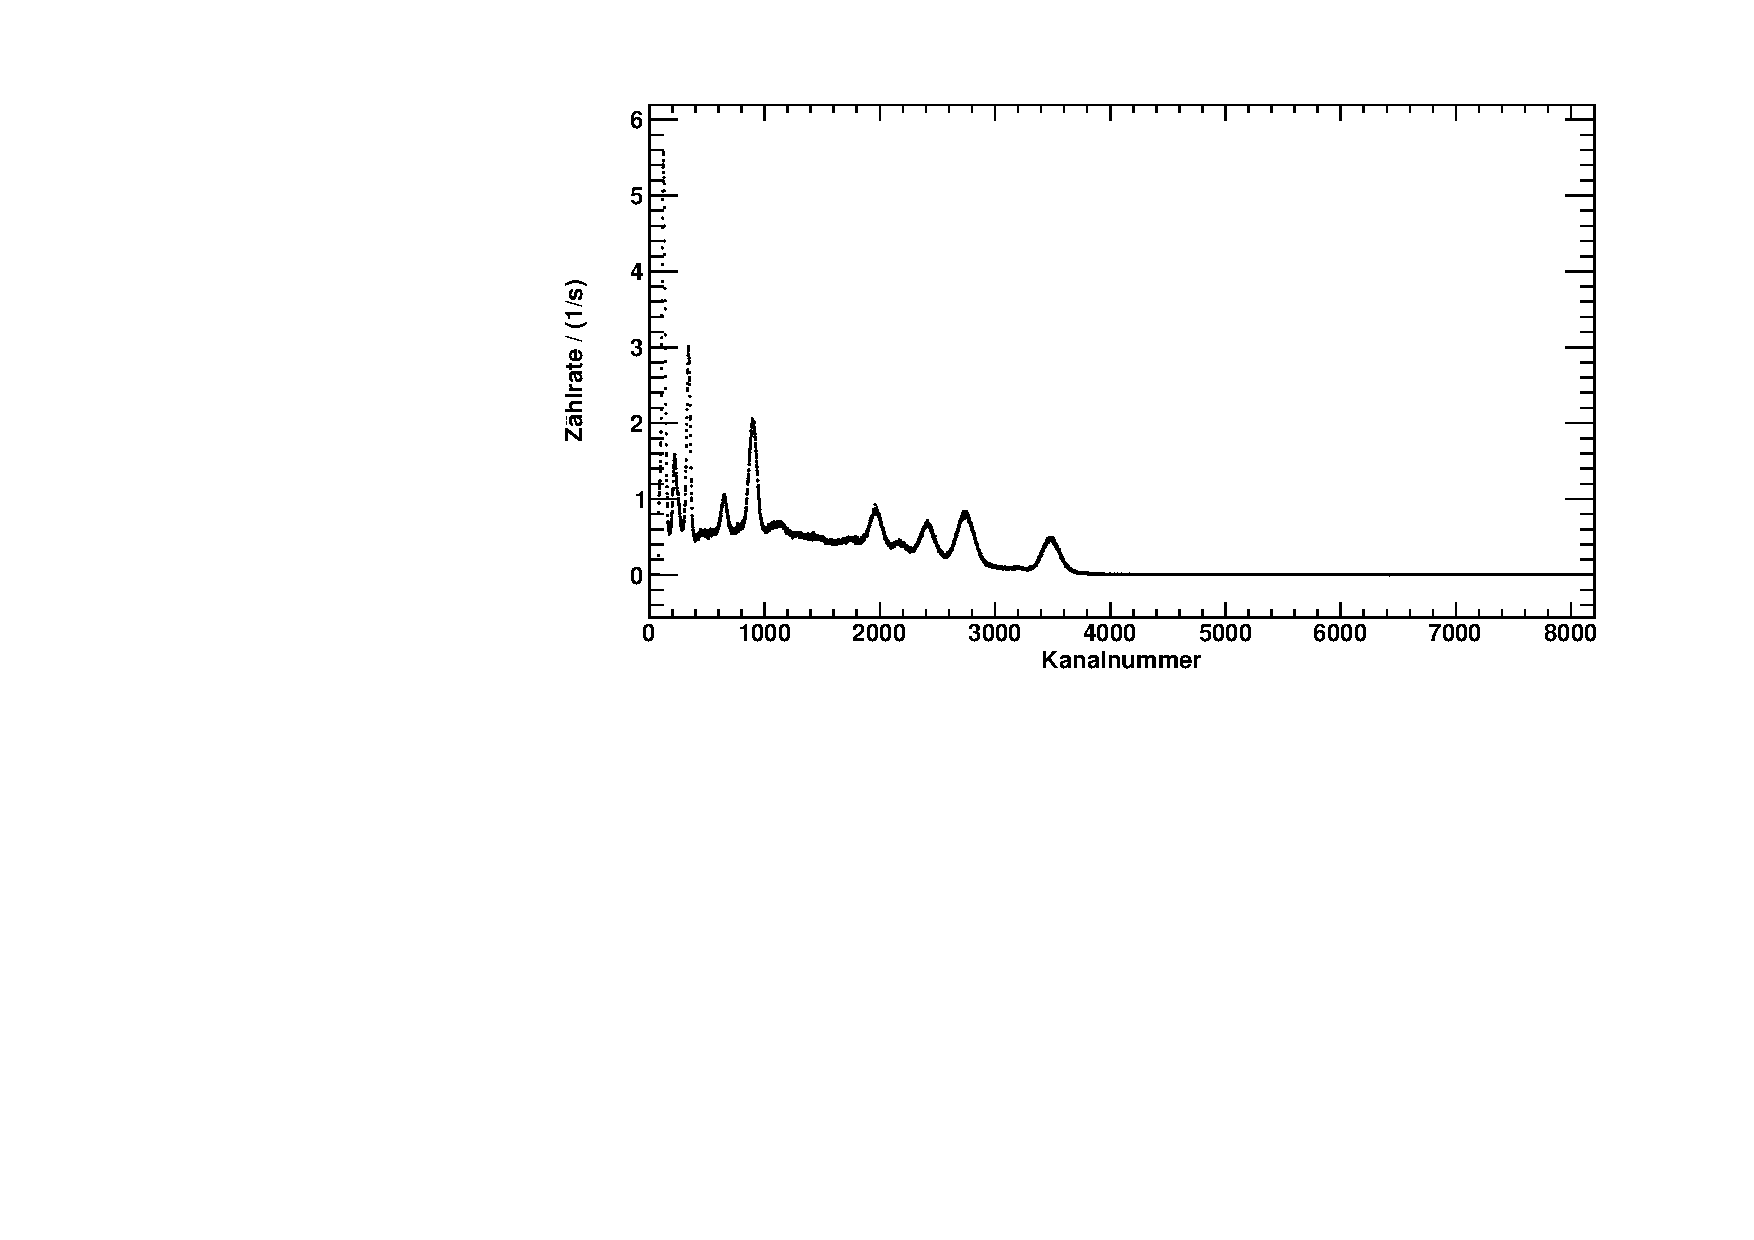
\includegraphics[width=\textwidth]{../img/eu_spectrum.pdf}
  \caption{\textgamma-spektrum von \chemel{Eu}{152}}
  \label{img:eu:spectrum}
\end{center}
\end{figure}
Die beiden Peaks wurden separat mit der gleichen Funktion wie bei \na\,(Kapitel \ref{subsub:eval:na}) gefittet:
\begin{equation}
  y_i = a_i + b_i \cdot x + \gaus(x; A_i, c_i, s_i), \qquad i = 1, 2
\end{equation}
Der Fit ist in \autoref{img:eu:peak} dargestellt und die Werte für die Peaks lauten:
\begin{equation}
\begin{split}
  \label{eq:eu:peaks}
  c_1 &= 340.41 \pm 0.07 \\
  c_2 &= 899.33 \pm 0.14
\end{split}
\end{equation}
\begin{figure}[H]
\begin{center}
  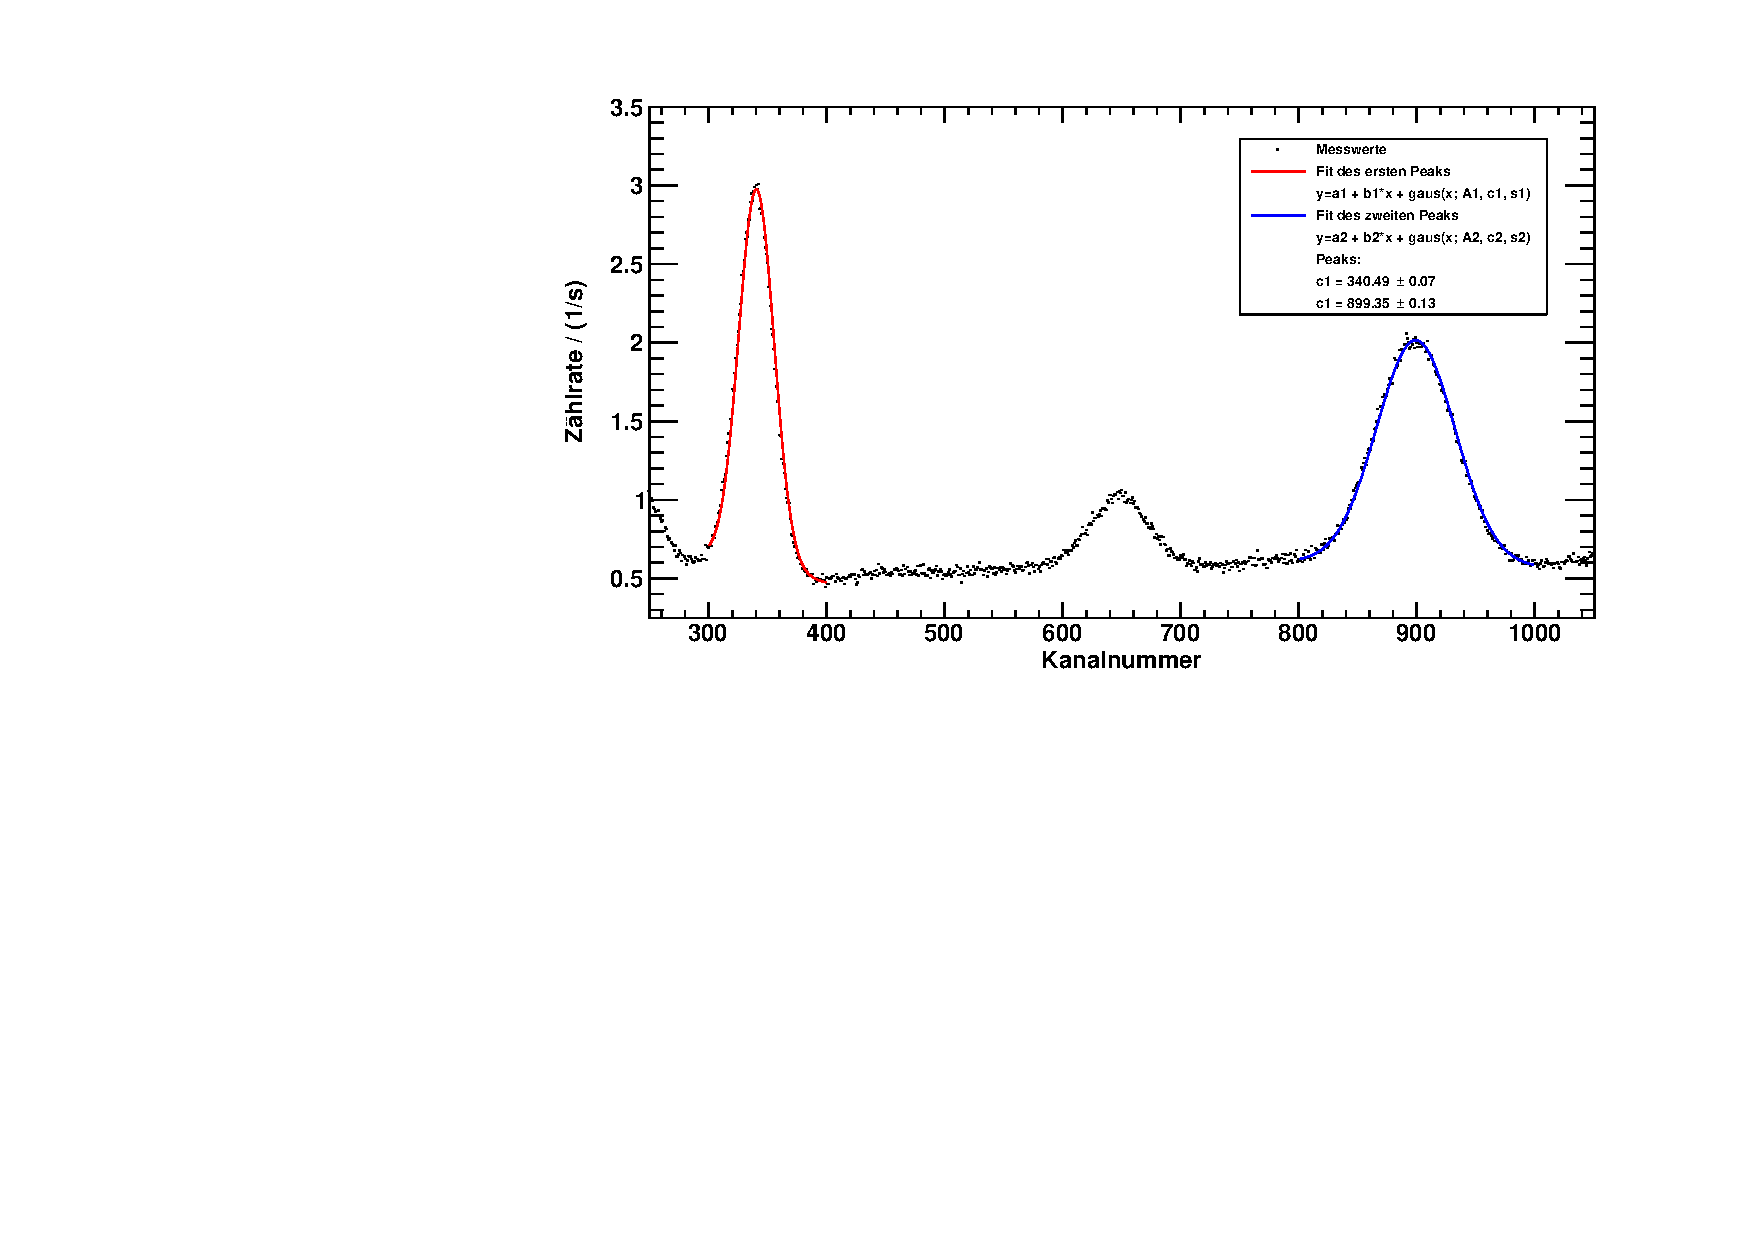
\includegraphics[width=\textwidth]{../img/eu_peaks.pdf}
  \caption{Fit der beiden Peaks (122\,keV und 344\,keV) von \eu\, mit jeweils einem linearen Untergrund und einer Gauß-Verteilung.}
  \label{img:eu:peak}
\end{center}
\end{figure}

\subsubsection{Energieeichung}
Die Werte für die Energieeichung aus Kapitel \ref{subsub:eval:na}, \ref{subsub:eval:co} und \ref{subsub:eval:eu} wurden in 
\autoref{tab:energygauge} zusammengefasst.
\begin{table}[H]
\caption{Referenzpeaks mit Literaturwerten}
\begin{center}
\begin{tabular}{|c|c|c|c|}
  \hline
  Element & Literaturwert / keV & Kanal & Fehler auf Kanal \\ \hline
  Na & 511 & 1302.38 & 1.66 \\ \hline
  Na & 1274 & 3135.85 & 4.69 \\ \hline
  Co & 1172 & 2897.27 & 0.53 \\ \hline
  Co & 1332 & 3283.30 & 0.57 \\ \hline
  Eu & 122 & 340.41 & 0.07 \\ \hline
  Eu & 344 & 899.33 & 0.14 \\ \hline
\end{tabular}
\end{center}
\label{tab:energygauge}
\end{table}

Es wurde zuerst ein linearer Fit durchgeführt, welcher in \autoref{img:gauge:lin} zu sehen ist.
\begin{equation}
  y = a + b\cdot x
\end{equation}
\label{subsub:energygauge}
\begin{figure}[H]
\begin{center}
  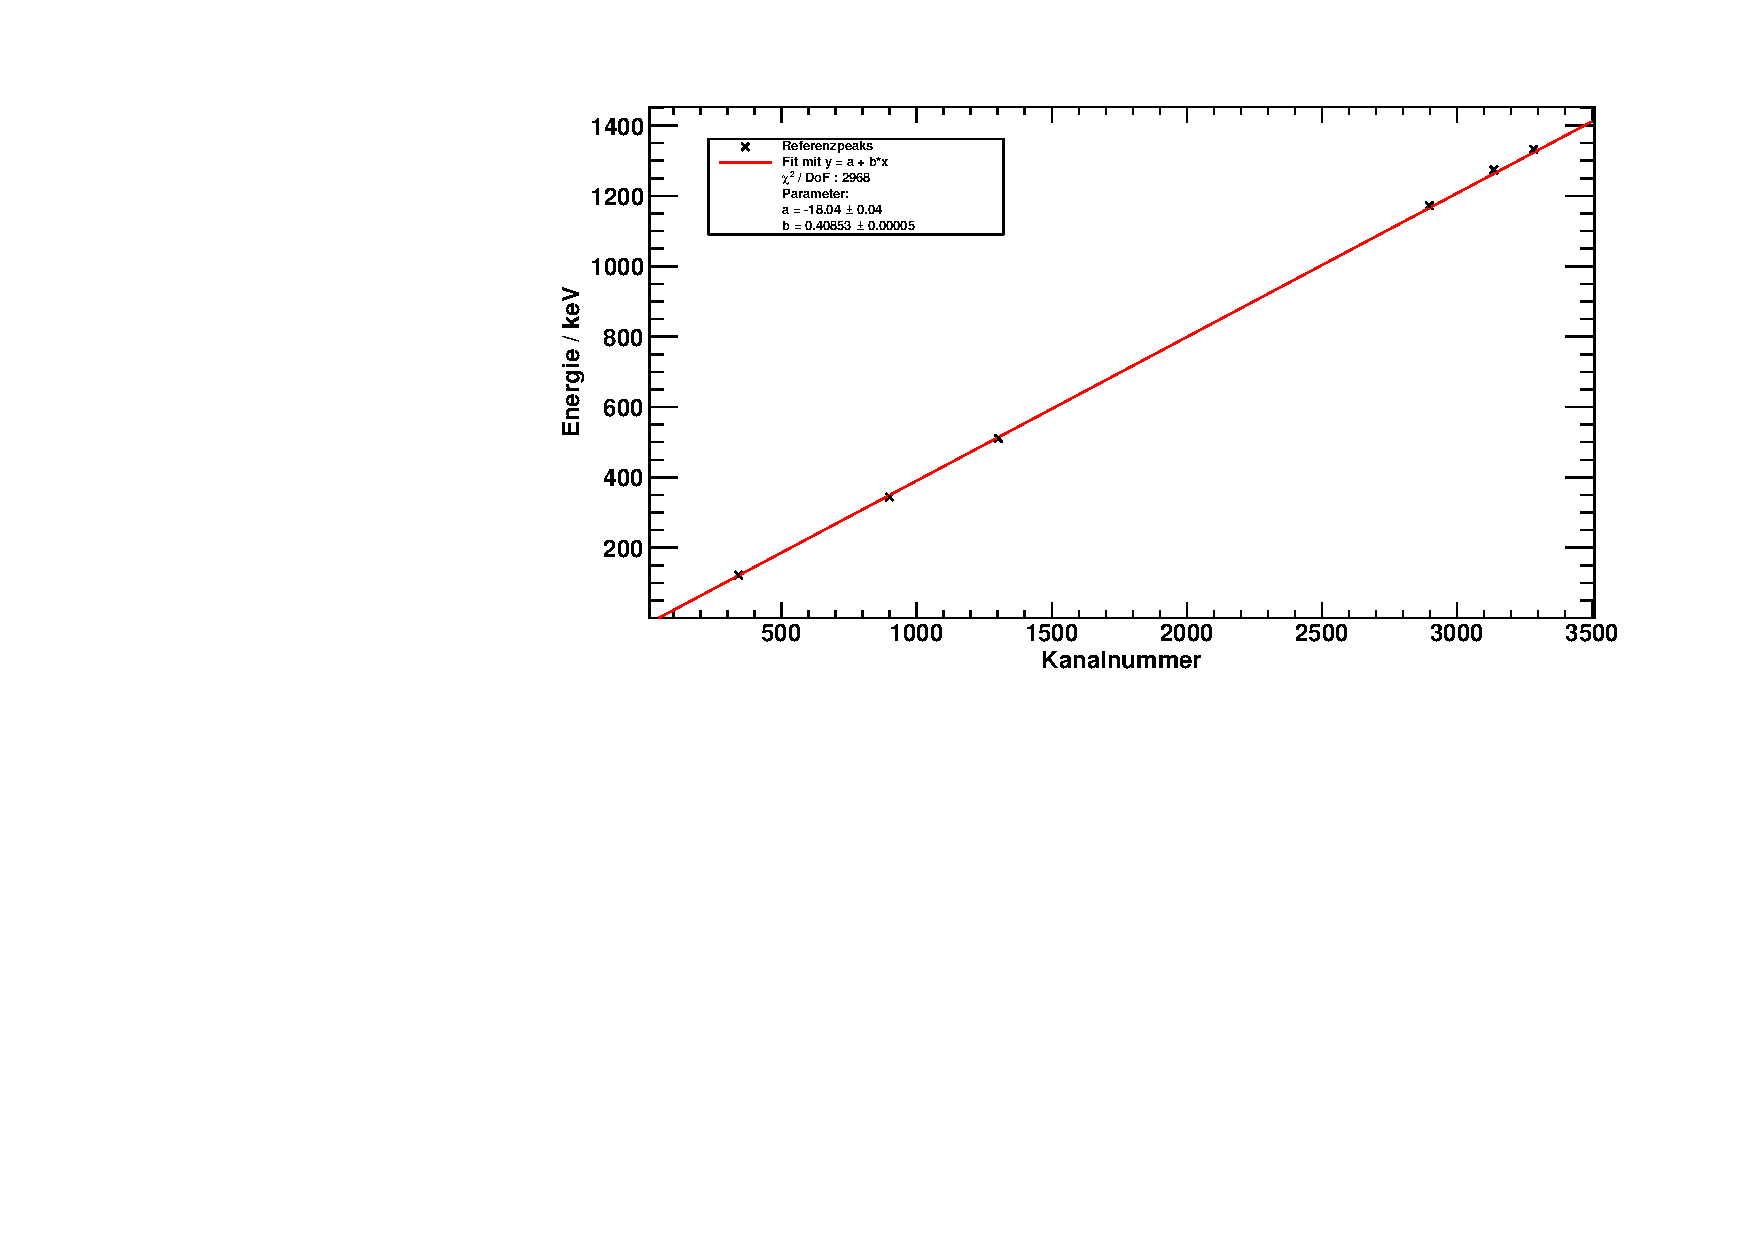
\includegraphics[width=\textwidth]{../img/energy_gauge_lin.pdf}
  \caption{Lineare Energieeichung}
  \label{img:gauge:lin}
\end{center}
\end{figure}
Allerdings erkennt man, dass der Fit die Daten nicht besonders gut beschreibt. Deshalb wurde ein Polynom zweiten Grades angesetzt:
\begin{equation}
  y = a + b\cdot x + c\cdot x^2
\end{equation}
Der Fit ist in \autoref{img:gauge:quad} dargestellt. Der Fit beschreibt nun besser die gemessenen Daten. Dies erkennt man auch, 
wenn man die $\chi^2$-Werte der beiden Graphen vergleicht. Das $\chi^2$ von dem linearen Fit beträgt ca. 2968, das des quadratischen Fits 
nur noch 95. Da den beiden Fits die gleichen Daten vorliegen, kann man diese beiden Werte gegenüberstellen\footnote{Dies ist im Allgemeinen nicht so,
da der $\chi^2$-Wert eines Fits von der y-Skalierung der gegebenen Daten abängt.}.
Die Parameter ergeben sich zu:
\begin{equation}
\begin{split}
  \label{eq:energygauge:params}
  a &= (-11.50 \pm 0.07) \,\text{keV} \\
  b &= (0.39004 \pm 0.00017) \,\text{keV} \\
  c &= (6.05 \pm 0.06) \cdot 10^{-6} \,\text{keV}
\end{split}
\end{equation}
mit Korrelationen
\begin{equation}
\begin{split}
  \label{eq:energygauge:corr}
  \rho_{a, b} &= -0.93 \, \frac{1}{\text{keV}^2} \\
  \rho_{a, c} &=  0.85 \, \frac{1}{\text{keV}^2} \\
  \rho_{b, c} &= -0.95 \, \frac{1}{\text{keV}^2} \\
\end{split}
\end{equation}
\begin{figure}[H]
\begin{center}
  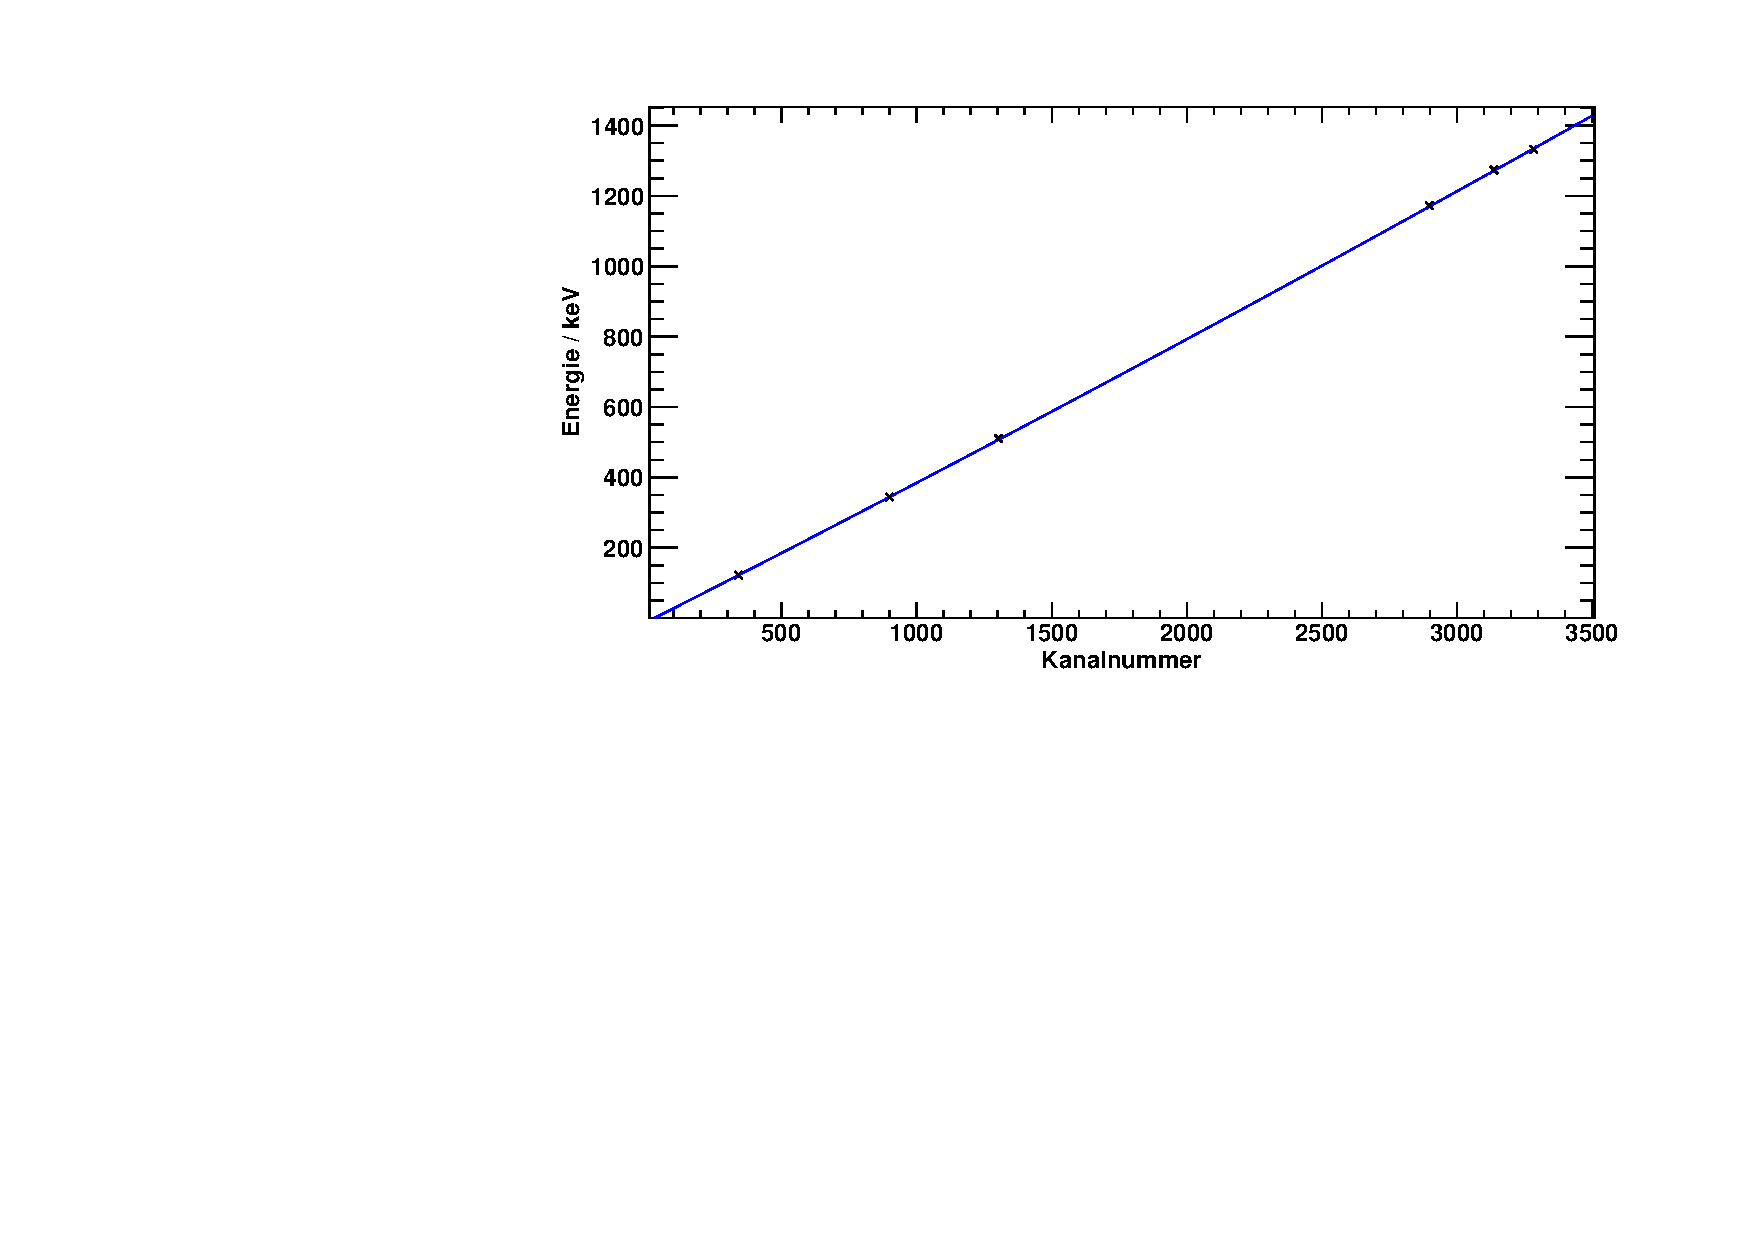
\includegraphics[width=\textwidth]{../img/energy_gauge_quad.pdf}
  \caption{Quadratische Energieeichung}
  \label{img:gauge:quad}
\end{center}
\end{figure}
Nun kann man einen Kanal $k$ in die entsprechende Energie umrechnen:
\begin{equation}
  \label{eq:energygauge}
  E(k) = a + b \cdot k + c \cdot k^2
\end{equation}
Der Fehler berechnet sich mit dem Gauß'schen Fehlerfortpflanzungsgesetz unter Berücksichtigung der Korrelationen:
\begin{equation}
	\label{eq:energygauge:error}
  s_E^2 = s_{k}^2 \cdot (b + 2 \cdot c \cdot k)^2 + 2 \cdot \rho_{a, b} \cdot s_{a} \cdot s_{b} \cdot k + 2 \cdot \rho_{a, c} \cdot s_{a} \cdot s_{c} \cdot k^2 +
  2 \cdot \rho_{b, c} \cdot s_{b} \cdot s_{c} \cdot k^3 + s_{a}^2 + s_{b}^2 \cdot k^2 + s_{c}^2 \cdot k^4
\end{equation}

\subsection{\textgamma-Spektrum von \th}
Das gesamte Spektrum von \th ist in \autoref{img:th:spectrum} zu sehen.
\begin{figure}[H]
\begin{center}
  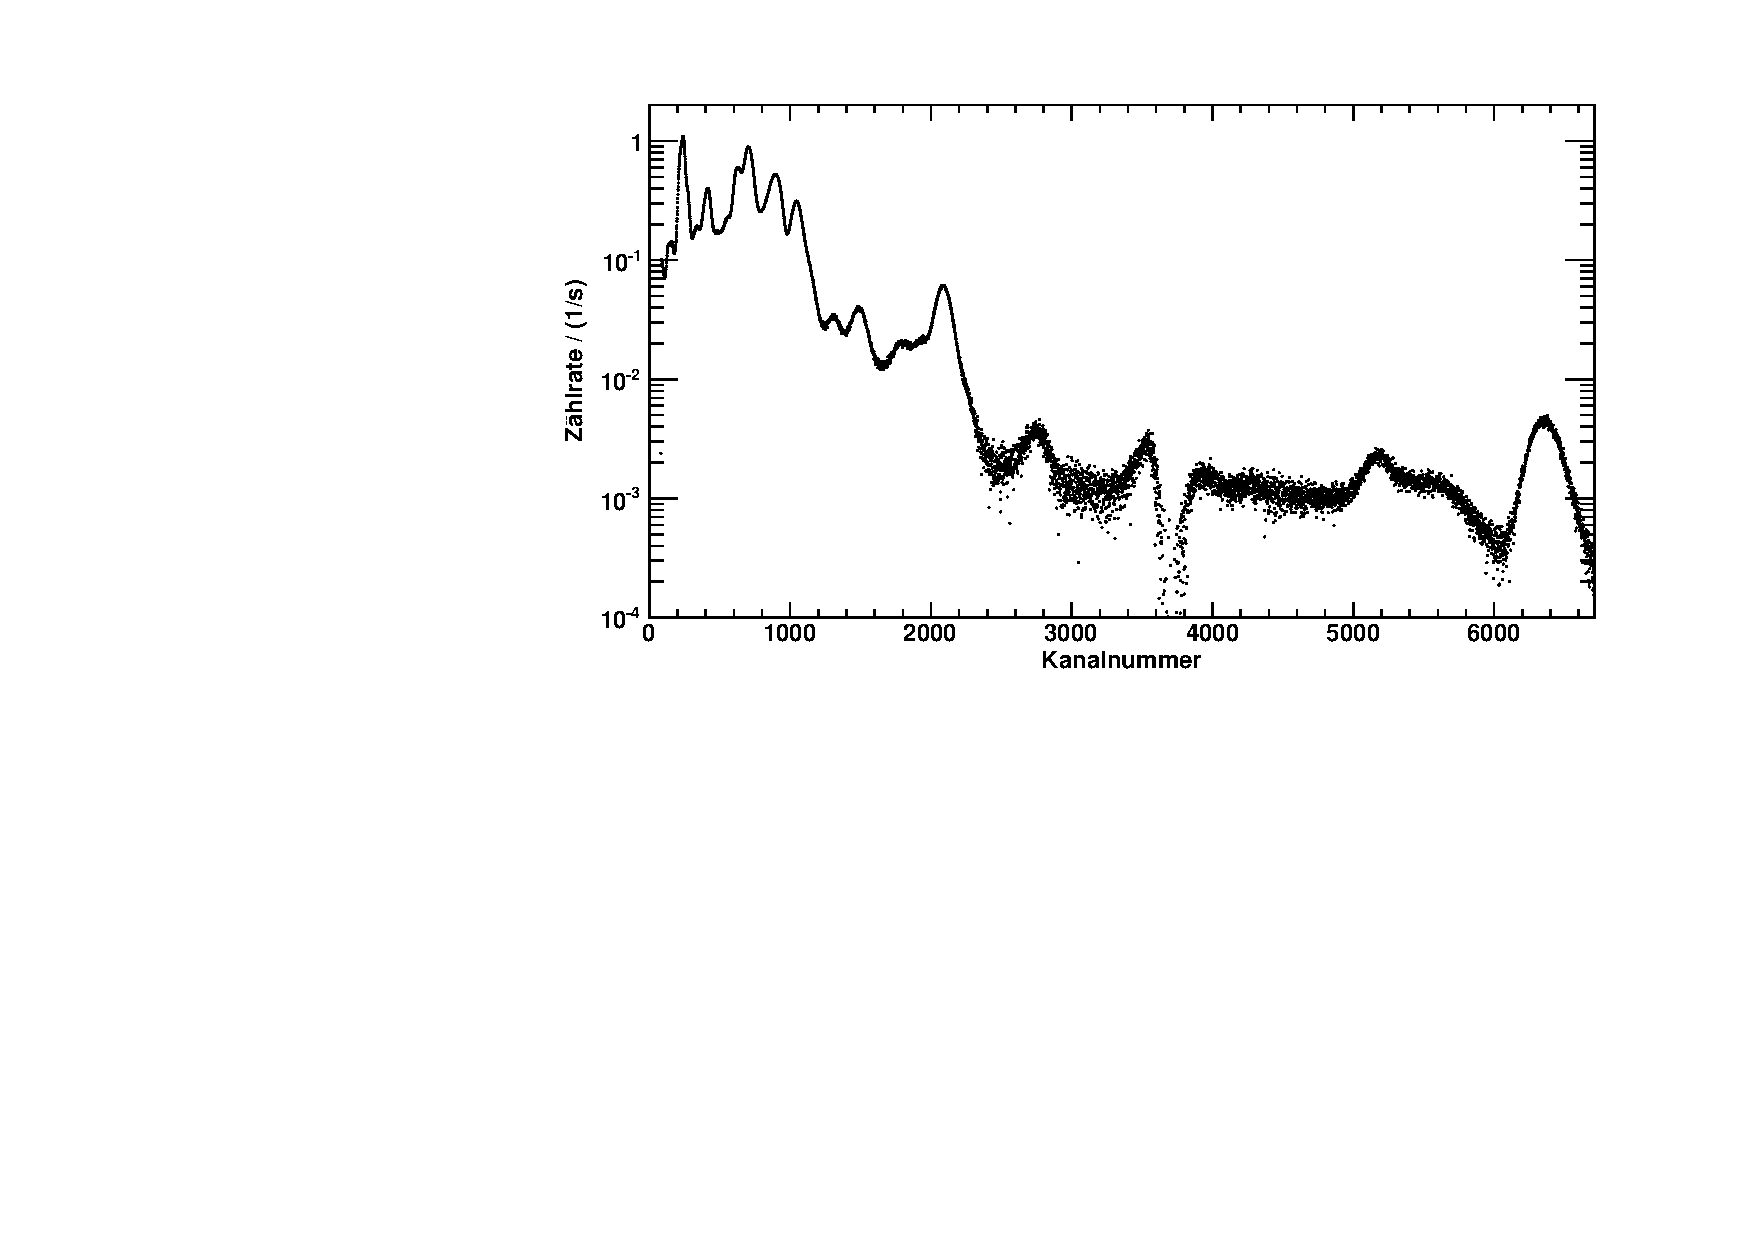
\includegraphics[width=\textwidth]{../img/th_energyspectrum.pdf}
  \caption{\textgamma-Spektrum von \th.}
  \label{img:th:spectrum}
\end{center}
\end{figure}
Man erkennt eine Vielzahl von Peaks, welche im Folgenden analysiert werden. Dazu wird zuerst jeder Peak separat betrachtet. Anschließend werden 
größere Gruppen von Peaks gemeinsam gefittet, um etwaige Überlagerungen zu berücksichtigen.

\subsubsection{Separate Betrachtung der Peaks}
Jeder der zehn erkennbaren Peak wird mit einer Gauß-Verteilung (\autoref{eq:gaus}) und einem linearen Untergrund gefittet.
\begin{equation}
  y_i = a_i + b_i \cdot x + \gaus(x; A_i, c_i, s_i), \qquad i=1, 2, \ldots, 10
\end{equation}
In \autoref{img:th:peaks:single:0106}, \autoref{img:th:peaks:single:0709} und \autoref{img:th:peaks:single:10} sind die einzelnen Fits der Peaks 
dargestellt.
\begin{figure}[H]
\begin{center}
  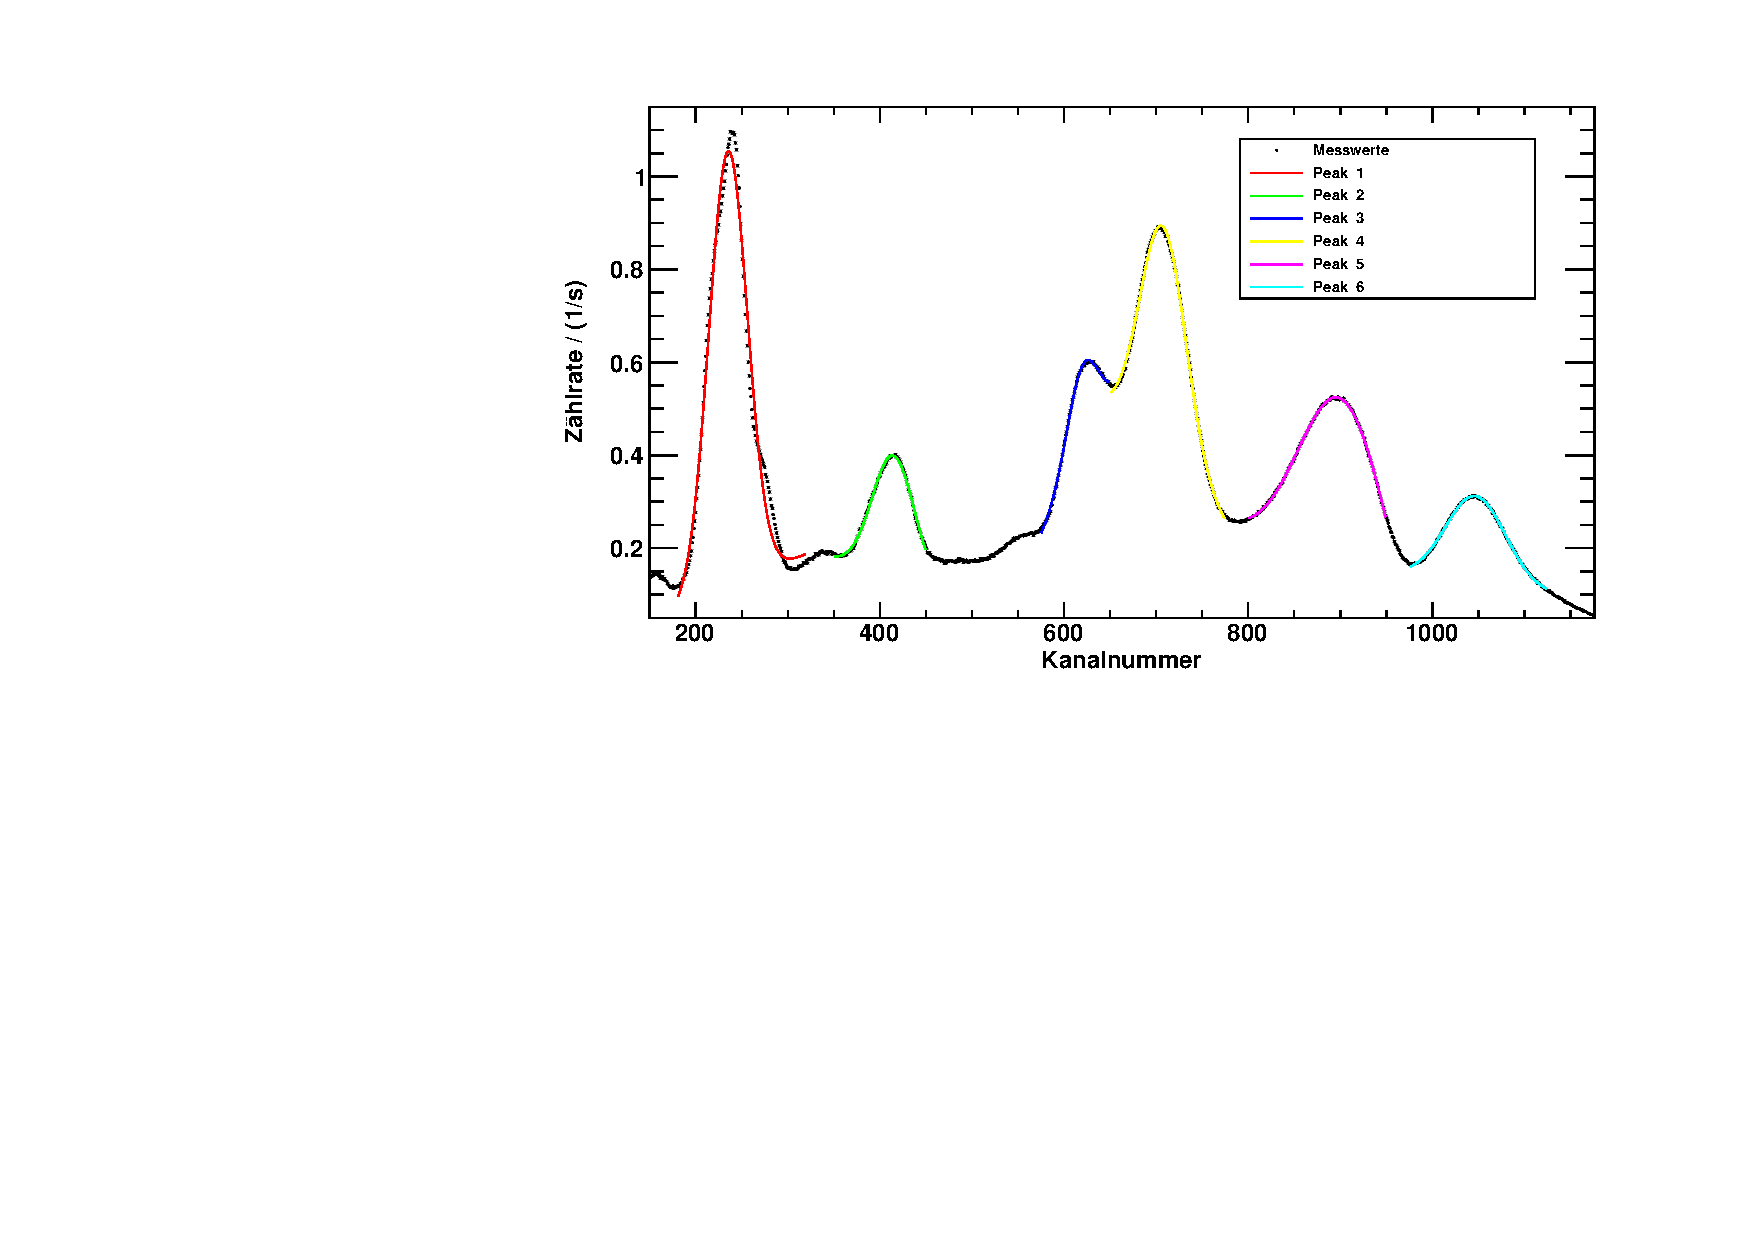
\includegraphics[width=\textwidth]{../img/th_peaks_single_01-06.pdf}
  \caption{Peaks 1 bis 6}
  \label{img:th:peaks:single:0106}
\end{center}
\end{figure}

\begin{figure}[H]
\begin{center}
  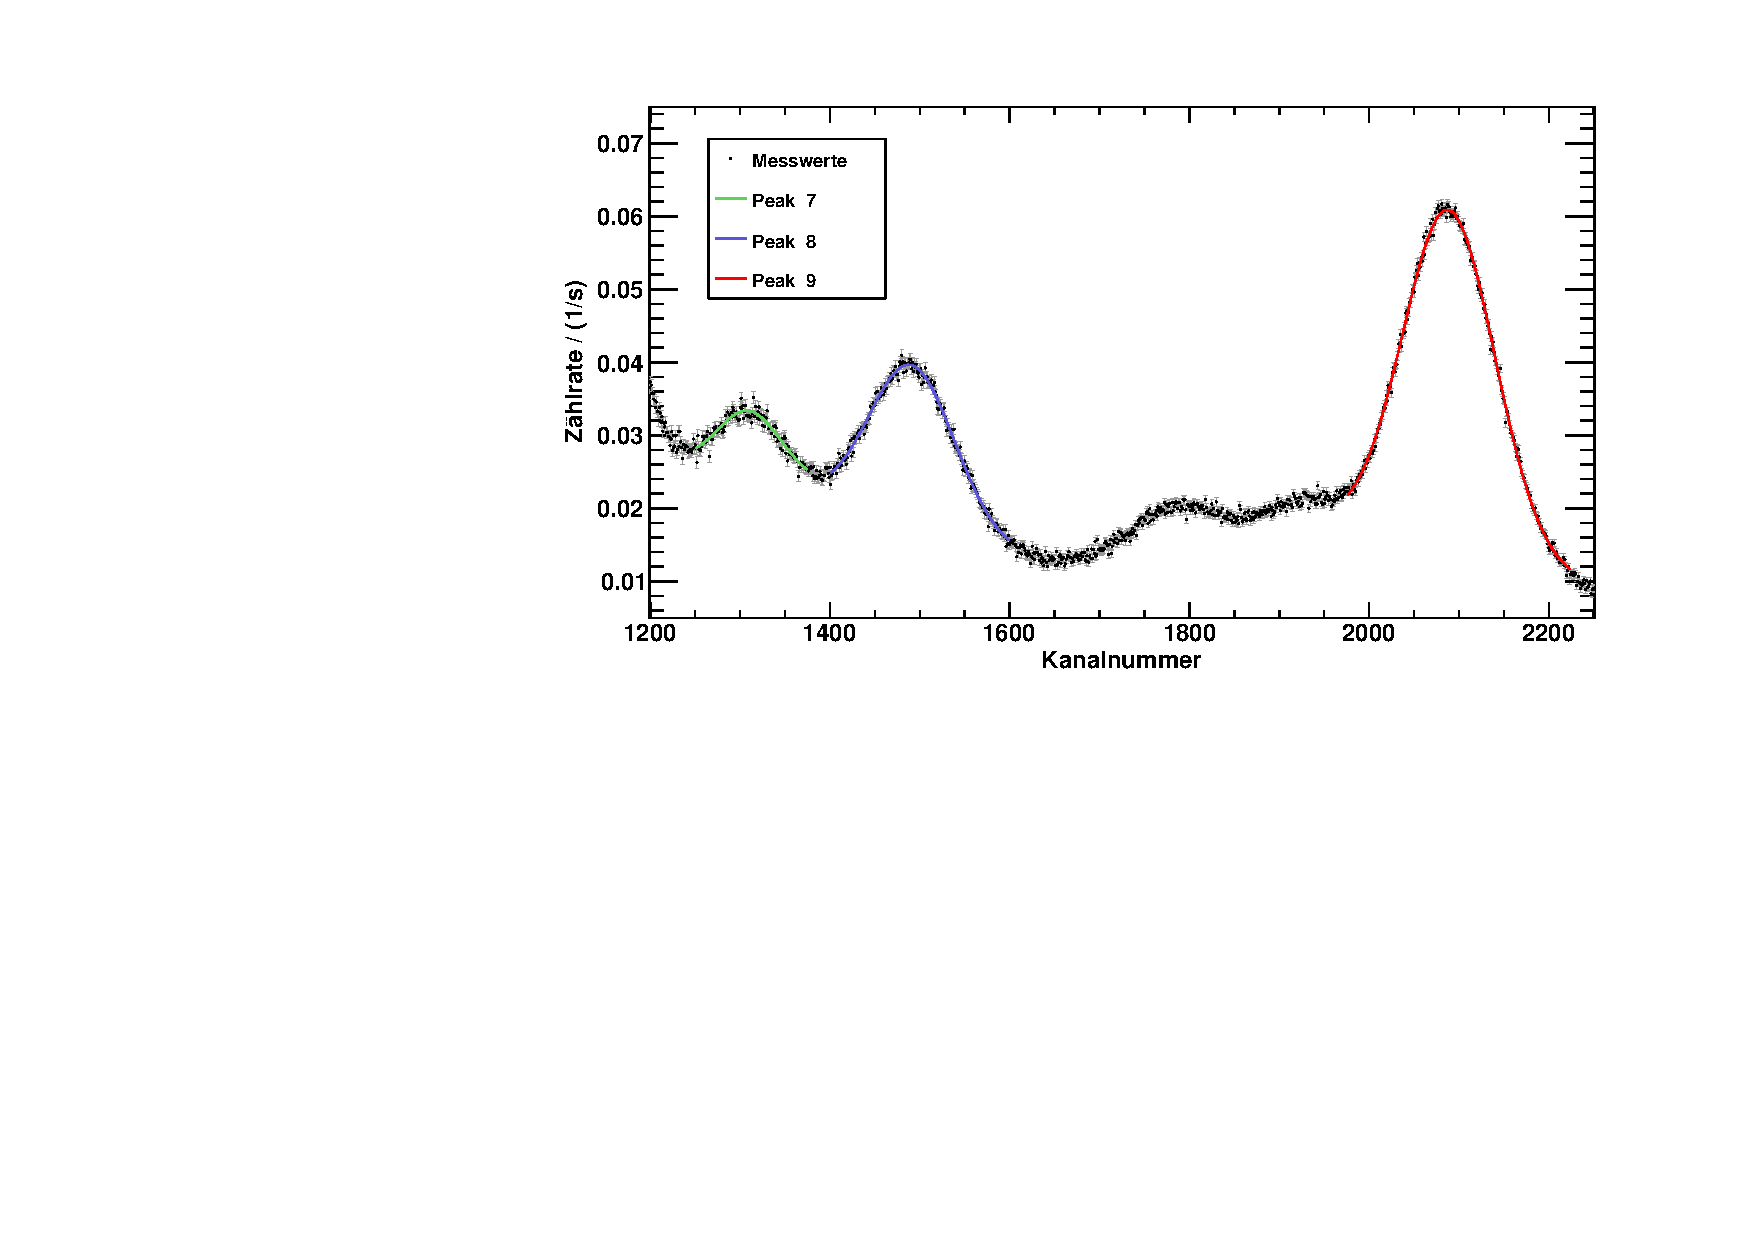
\includegraphics[width=\textwidth]{../img/th_peaks_single_07-09.pdf}
  \caption{Peaks 7 bis 9}
  \label{img:th:peaks:single:0709}
\end{center}
\end{figure}

\begin{figure}[H]
\begin{center}
  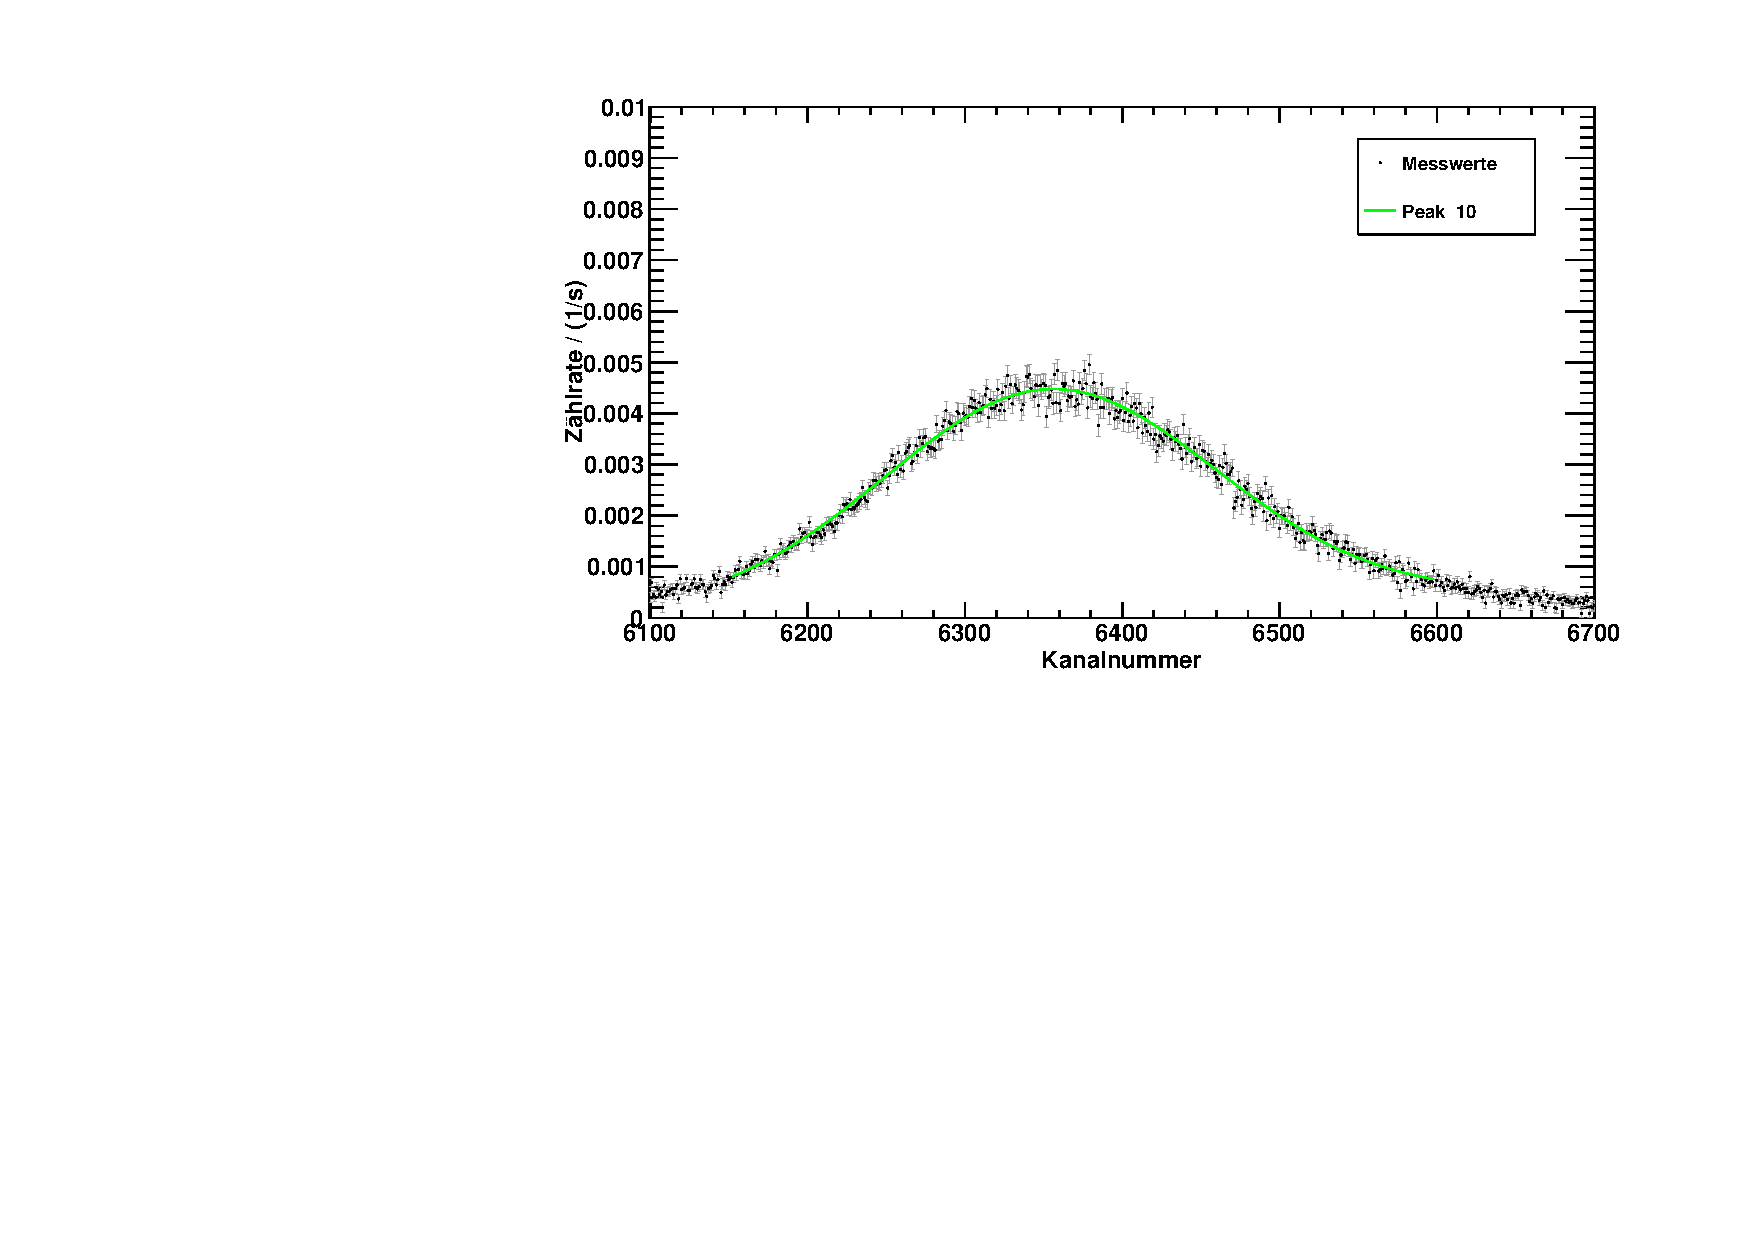
\includegraphics[width=\textwidth]{../img/th_peaks_single_10.pdf}
  \caption{Peak 10}
  \label{img:th:peaks:single:10}
\end{center}
\end{figure}

Die Ergebnisse der Fits und die zugehörigen Energien (entsprechend \autoref{eq:energygauge}) sind in \autoref{tab:th:single} aufgelistet.
Der große Fehler auf den Kanal bei Peak 7 könnte sich durch einen Doppelpeak, der sich nicht mehr auflösen lässt, erklären.
\begin{table}[H]
\caption{Kan\"ale und Energien von \th, bestimmt mit separaten Fits.}
\begin{center}
\begin{tabular}{|c|c|c|c|c|}
  \hline
   & Kanal c & $s_c$ & Energie $E$ / keV & $s_E$ / keV \\ \hline
  Peak 1 & 235.190 & 0.017 & 80.57 & 0.12 \\ \hline
  Peak 2 & 414.734 & 0.122 & 151.31 & 0.31 \\ \hline
  Peak 3 & 620.090 & 0.112 & 232.69 & 0.30 \\ \hline
  Peak 4 & 707.534 & 0.034 & 267.50 & 0.17 \\ \hline
  Peak 5 & 905.922 & 0.319 & 346.82 & 0.51 \\ \hline
  Peak 6 & 1046.990 & 0.066 & 403.51 & 0.24 \\ \hline
  Peak 7 & 1309.927 & 1.525 & 509.81 & 1.12 \\ \hline
  Peak 8 & 1491.048 & 0.501 & 583.53 & 0.65 \\ \hline
  Peak 9 & 2088.713 & 0.166 & 829.59 & 0.38 \\ \hline
  Peak 10 & 6354.170 & 0.780 & 2711.20 & 1.55 \\ \hline
\end{tabular}
\end{center}
\label{tab:th:single}
\end{table}


\subsubsection{Multi-Peak Fit} % TODO Benennung
Da die Peaks 1 bis 6 und 7 bis 8 nahe beieinander liegen, könnte ein gemeinsamer Fit der Peaks gegenseitige Einflüsse ausgleichen.
Dazu wird ein quadratischer Untergrund angesetzt und über die verschieden Gauß-Verteilungen der Peaks summiert:
\begin{equation}
  y = a + b\cdot x + c\cdot x^2 + \sum_{i=N_0}^{N} \gaus(x; A_i, c_i, s_i)
\end{equation}
wobei $N_0$ den ersten und $N$ den letzten Peak bezeichnet. Als Startparameter für den Fit wurden die Ergebnisse der separaten Fits benutzt.\\
Der Fit für die Peaks 1 bis 6 ist in \autoref{img:th:peaks:multi:0106} und der Fit für Peak 7 und 8 in 
\autoref{img:th:peaks:multi:0708} dargestellt.
\begin{figure}[H]
\begin{center}
  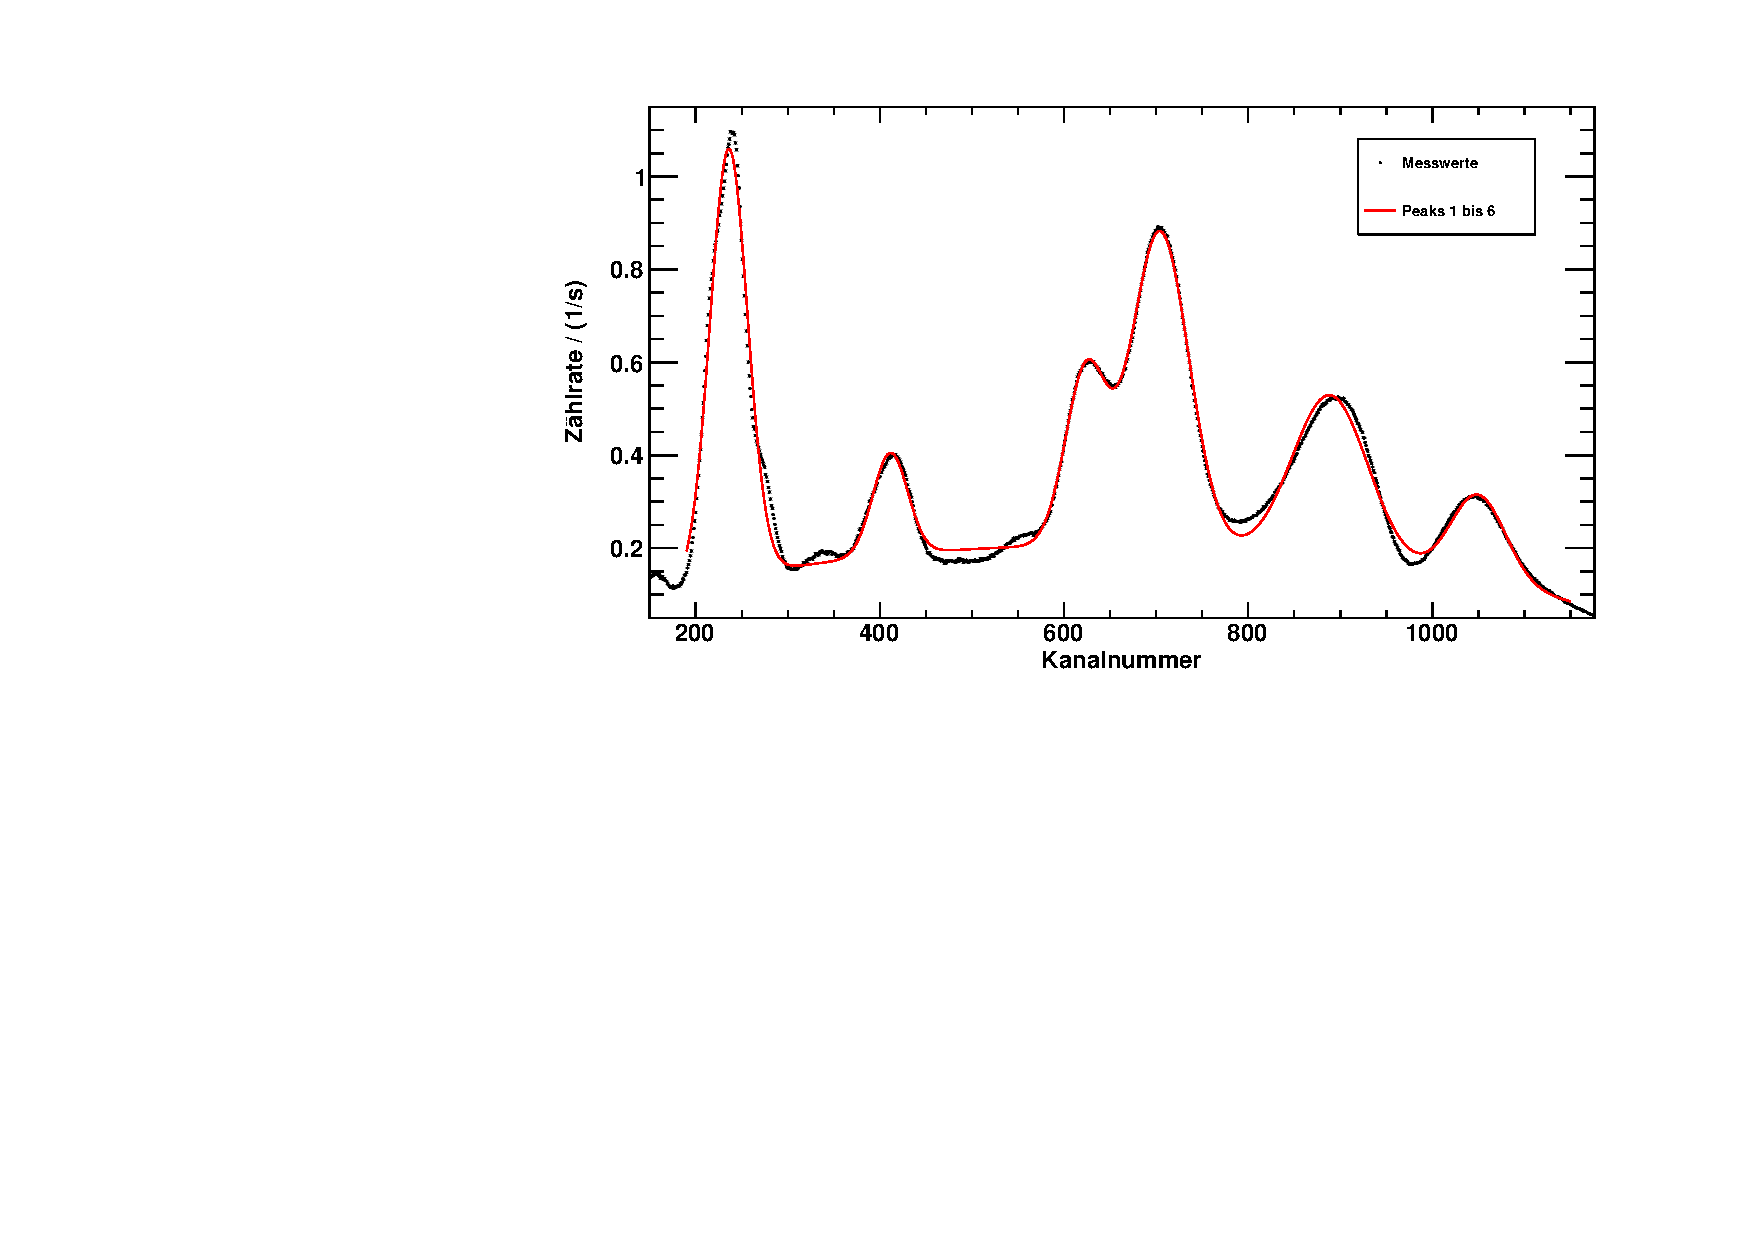
\includegraphics[width=\textwidth]{../img/th_peaks_multi_01-06.pdf}
  \caption{Peaks 1 bis 6}
  \label{img:th:peaks:multi:0106}
\end{center}
\end{figure}

\begin{figure}[H]
\begin{center}
  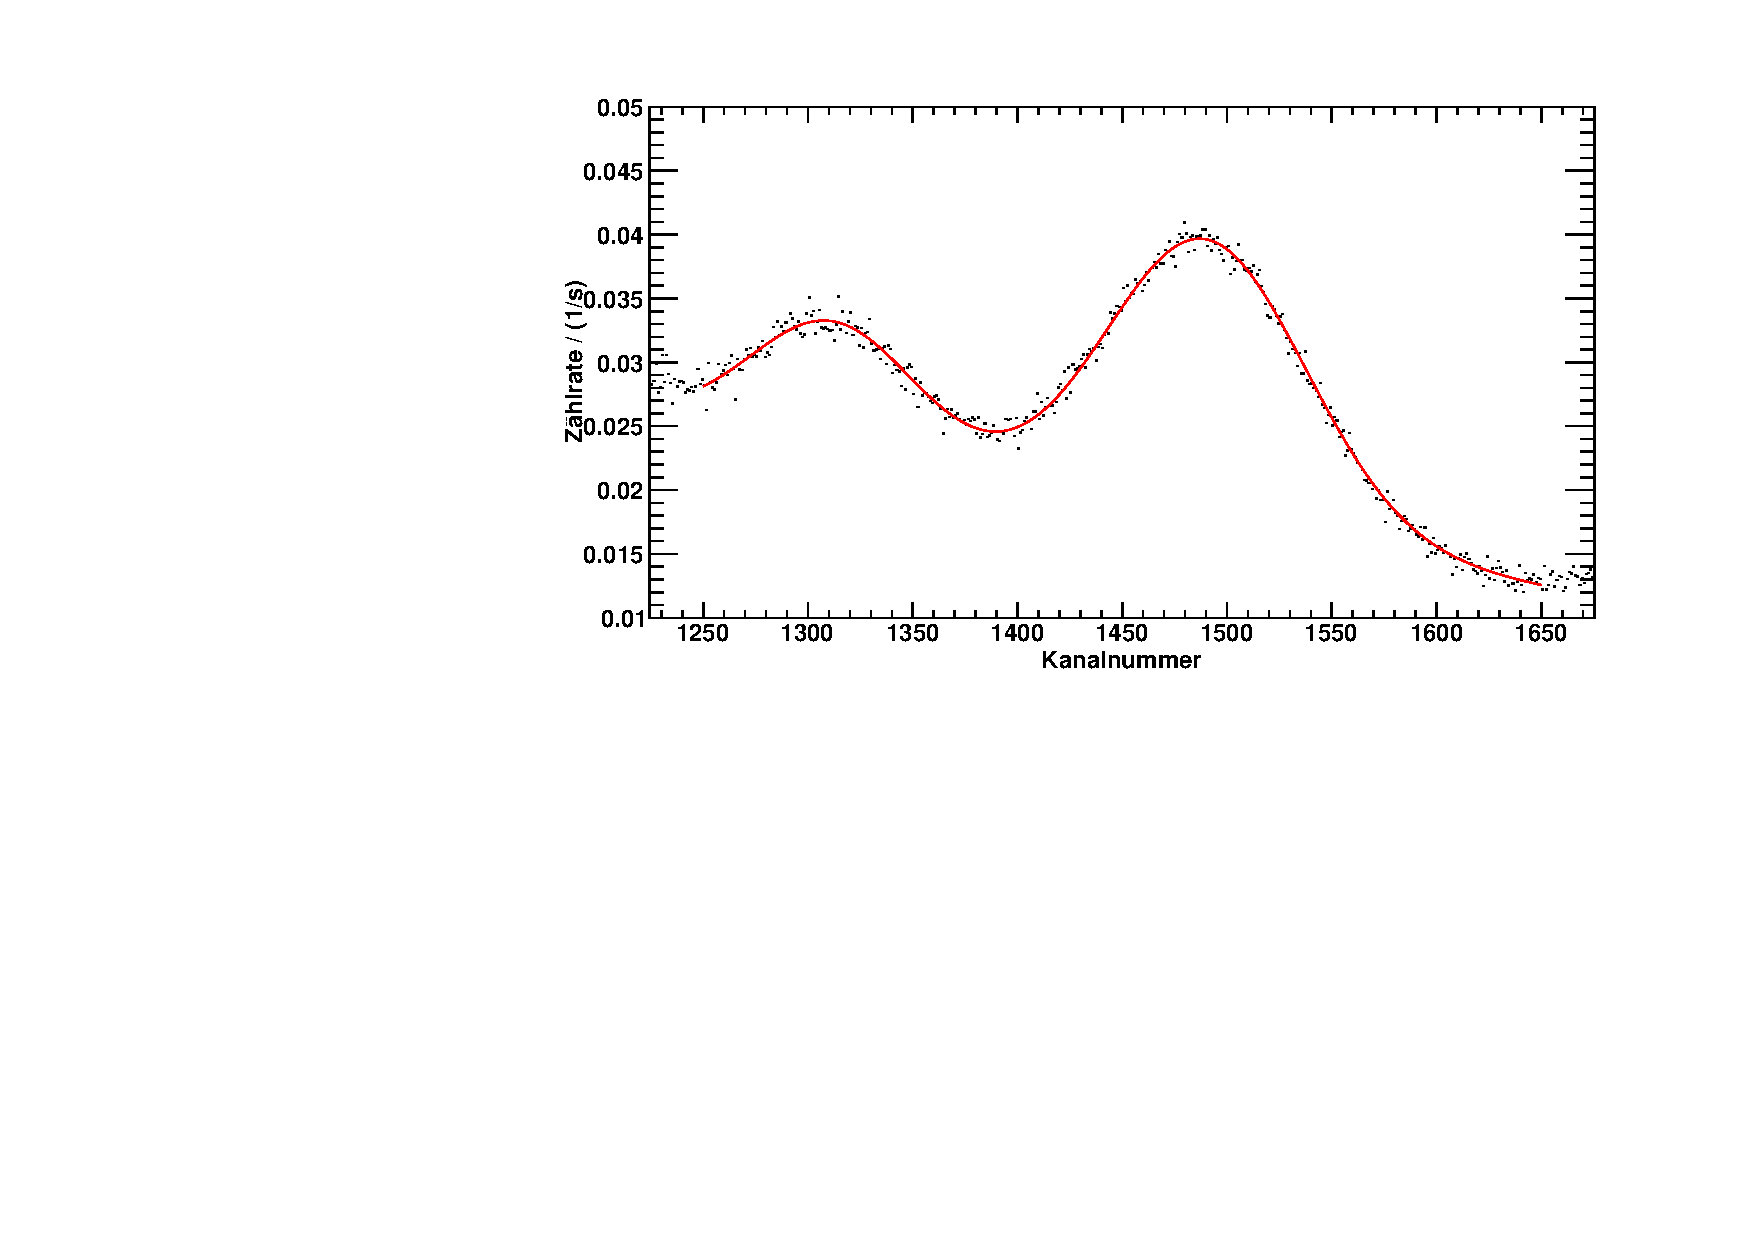
\includegraphics[width=\textwidth]{../img/th_peaks_multi_07-08.pdf}
  \caption{Peaks 7 und 8}
  \label{img:th:peaks:multi:0708}
\end{center}
\end{figure}
Die Werte für die Kanäle der Peaks und die entsprechenden Energien sind in \autoref{tab:th:multi} dargestellt. Diese Werte sind genauer, da sie 
gegenseitige Einflüsse berücksichtigen und werden in der Zuordnung verwendet.
\begin{table}[H]
\caption{Kan\"ale und Energien von \th, bestimmt mit gemeinsamen Fits.}
\begin{center}
\begin{tabular}{|c|c|c|c|c|}
  \hline
  Peak & Kanal $c$ & $s_c$ & Energie $E$ / keV & $s_E$ / keV \\ \hline
   1 & 235.864 & 0.015 & 80.84 & 0.11 \\ \hline
   2 & 411.342 & 0.046 & 149.97 & 0.19 \\ \hline
   3 & 623.715 & 0.045 & 234.13 & 0.19 \\ \hline
   4 & 704.111 & 0.029 & 266.14 & 0.16 \\ \hline
   5 & 889.061 & 0.033 & 340.06 & 0.17 \\ \hline
   6 & 1049.781 & 0.041 & 404.63 & 0.19 \\ \hline
   7 & 1312.604 & 0.578 & 510.90 & 0.69 \\ \hline
   8 & 1489.981 & 0.270 & 583.09 & 0.48 \\ \hline
\end{tabular}
\end{center}
\label{tab:th:multi}
\end{table}


\subsubsection{Zuordnung der Peaks}
Für Peak 1 bis 8 wurden die Werte der gemeinsamen Fits genommen, die Werte von Peak 9 und 10 stammen aus den separaten Fits.
Die Zuordung wurde in \autoref{tab:assign} durchgeführt.\\[\baselineskip]
\begin{table}
\caption{Zuordung der Peaks zu den Elementen}
\begin{center}
\begin{tabularx}{\textwidth}{|c|c|X|}
  \hline 
    Peak & $E$ / keV & Kernenergieniveaus und Tochterkern des Zerfalls, Literaturwert \\ \hline
      1 & $  80.84 \pm 0.11 $ &  $\gamma_{1,0}(\text{Ra})$, $84.373$\,keV \\ \hline
      2 & $ 149.97 \pm 0.16 $ &  $\gamma_{2,1}(\text{Ra})$, $131.612$\,keV oder $\gamma_{3,1}(\text{Ra})$, $166.41$\,keV \\ \hline
      3 & $ 234.13 \pm 0.19 $ &  $\gamma_{2,0}(\text{Ra})$, $215.985$\,keV \\ \hline
      4 & $ 266.14 \pm 0.16 $ &  $\gamma_{1,0}(\text{Rn})$, $240.986$\,keV oder $\gamma_{2,0}(\text{Bi})$, $238.637$\,keV \\ \hline
      5 & $ 340.06 \pm 0.17 $ &  $\gamma_{3,1}(\text{Bi})$, $300.09$\,keV \\ \hline
      6 & $ 404.63 \pm 0.19 $ &  $\gamma_{4,1}(\text{Tl})$, $452.8$\,keV \\ \hline
      7 & $ 510.9  \pm 0.7  $ &  $\gamma_{4,2}(\text{Pb})$, $510.7$\,keV \\ \hline
      8 & $ 583.1  \pm 0.5  $ &  $\gamma_{2,1}(\text{Pb})$, $583.187$\,keV \\ \hline
      9 & $ 829.6  \pm 0.4  $ &  $\gamma_{1,0}(\text{Pb})$, $804.9$\,keV \\ \hline
     10 & $ 2711.2 \pm 1.6  $ &  $\gamma_{1,0}(\text{Pb})$, $2614.511$\,keV \\ \hline
\end{tabularx}
\end{center}
\label{tab:assign}
\end{table}
Die Zuordnung wurde unter Berücksichtigung der Intensitäten der einzelnen Übergänge und Position im Spektrum durchgeführt. Die Literaturwerte 
wurden aus der Kemkartei übernommen (Auzüge im Anhang der Vorbereitung). Es fällt auf, dass einige Werte sehr genau mit den Literaturwerten 
übereinstimmen (z.B. Peak 7 und 8). Für andere lies sich kein besserer Literaturwert finden. Unter der Annahme der Korrektheit der Zuordnungen wäre 
eine Erklärung für die hohe Diskrepanz Verschiebung der Maxima aufgrund von Comptonstreuung höherenergetischer Photonen.

\subsection{Untergrundpeak}
\label{sub:eval:undergroundpeak}

\begin{figure}[H]
\begin{center}
  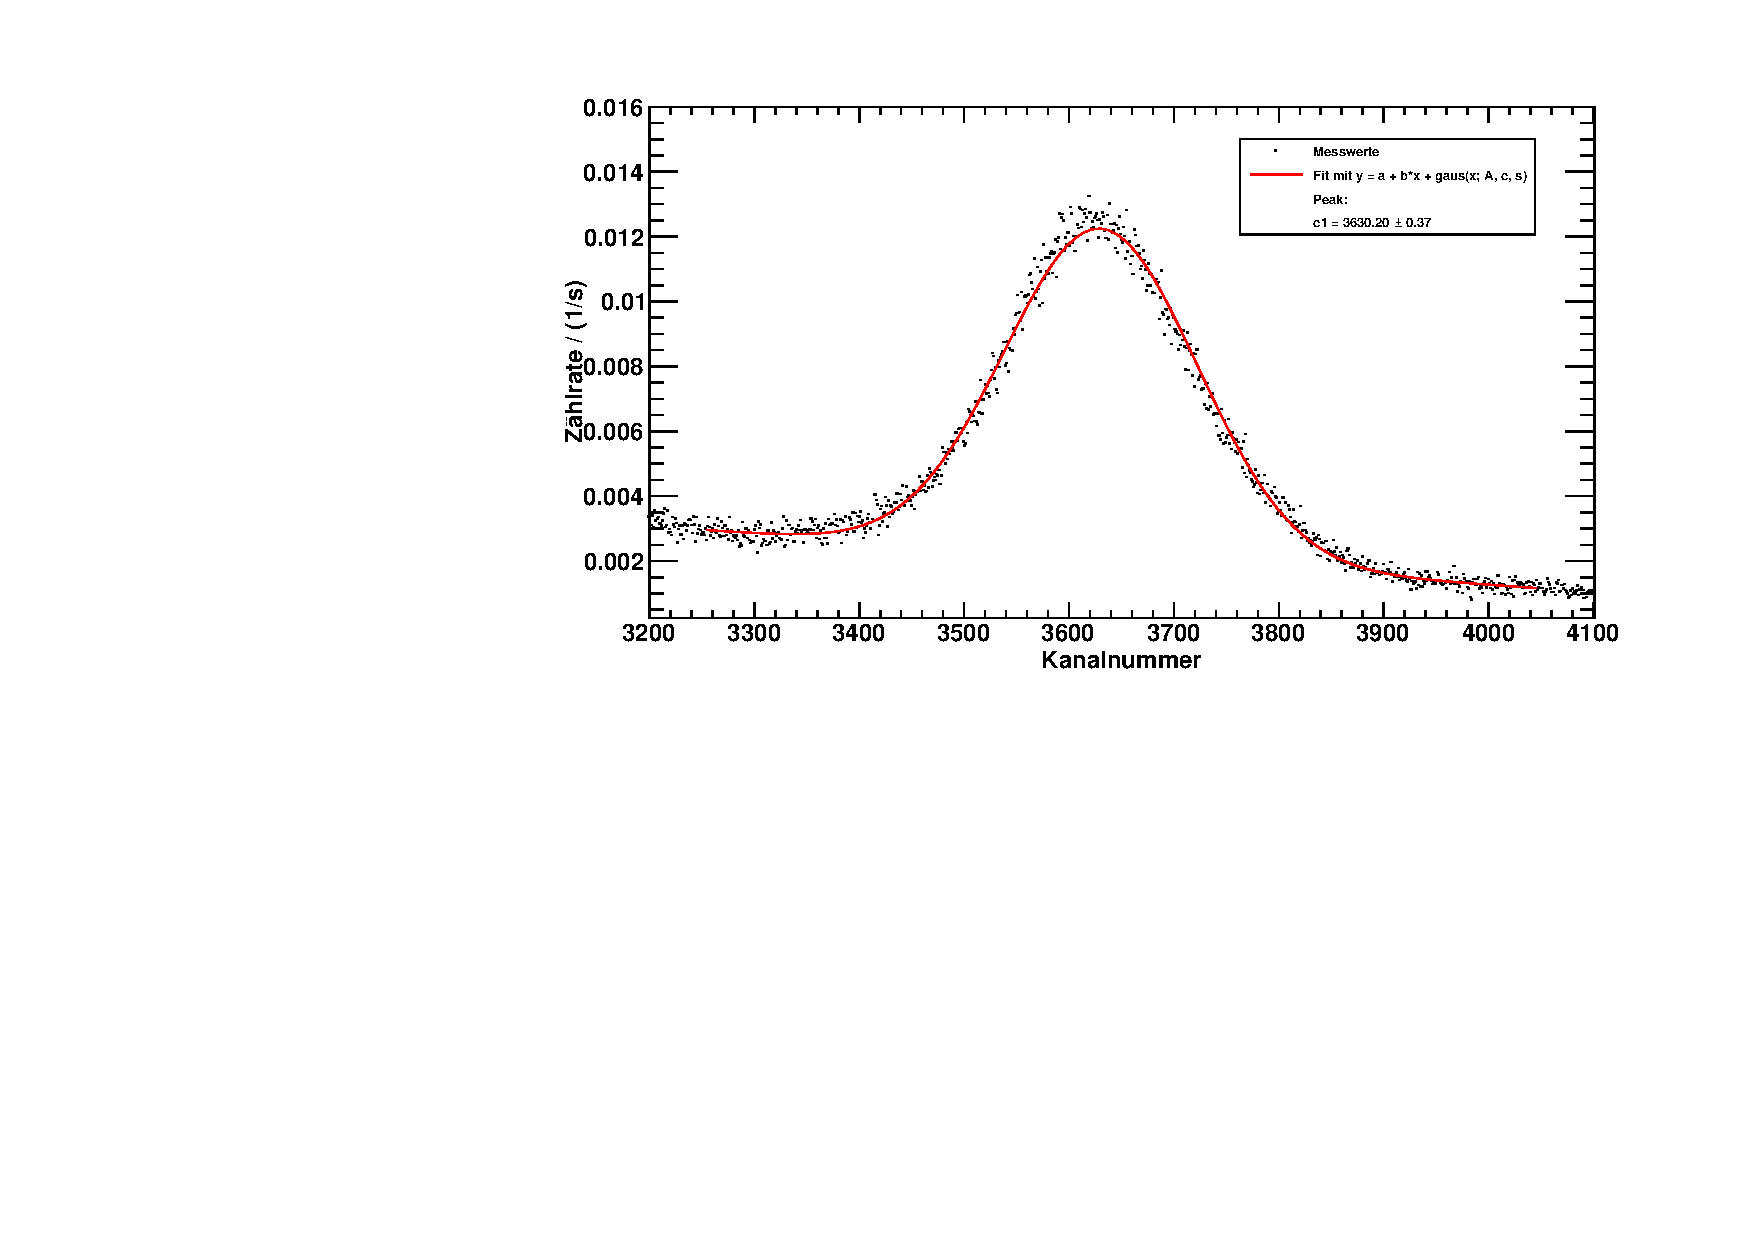
\includegraphics[width=\textwidth]{../img/underground_peaks.pdf}
  \caption{\chemel{Ka}{40}-Peak in der Untergrundmessung, Vergrößerung aus \autoref{img:underground:spectrum}.}
  \label{img:eval:undergroundpeak}
\end{center}
\end{figure}

\autoref{img:eval:undergroundpeak} zeigt vergrößert
den markanten Peak des Untergrunds von \autoref{img:underground:spectrum}.
Mit den Ergebnissen der Energieeichung kann auch hier jetzt die Energie der Strahlung bestimmt werden.
Wie oben wurde eine Gaußkurve über linearem Untergrund angepasst:
\begin{equation}
  y = a + b \cdot x + \gaus(x, A, c, s)
\end{equation}
Für das Zentrum der Verteilung $c_{\,{}^{40}\text{Ka}}$ erhält man aus dem Fit
\begin{equation}
  c_{\,{}^{40}\text{Ka}} = 3630.2 \pm 0.4	
\end{equation}
und damit für die Energie $E_{\,{}^{40}\text{Ka}}$ gemäß \autoref{eq:energygauge} und \autoref{eq:energygauge:error}
\begin{equation}
  E_{\,{}^{40}\text{Ka}} = (1484.2 \pm 0.6)\,\text{keV}
\end{equation}
\subsection{Winkelkorrelation der \chemel{Na}{22} Vernichtungsphotonen}
\begin{figure}[H]
\begin{center}
  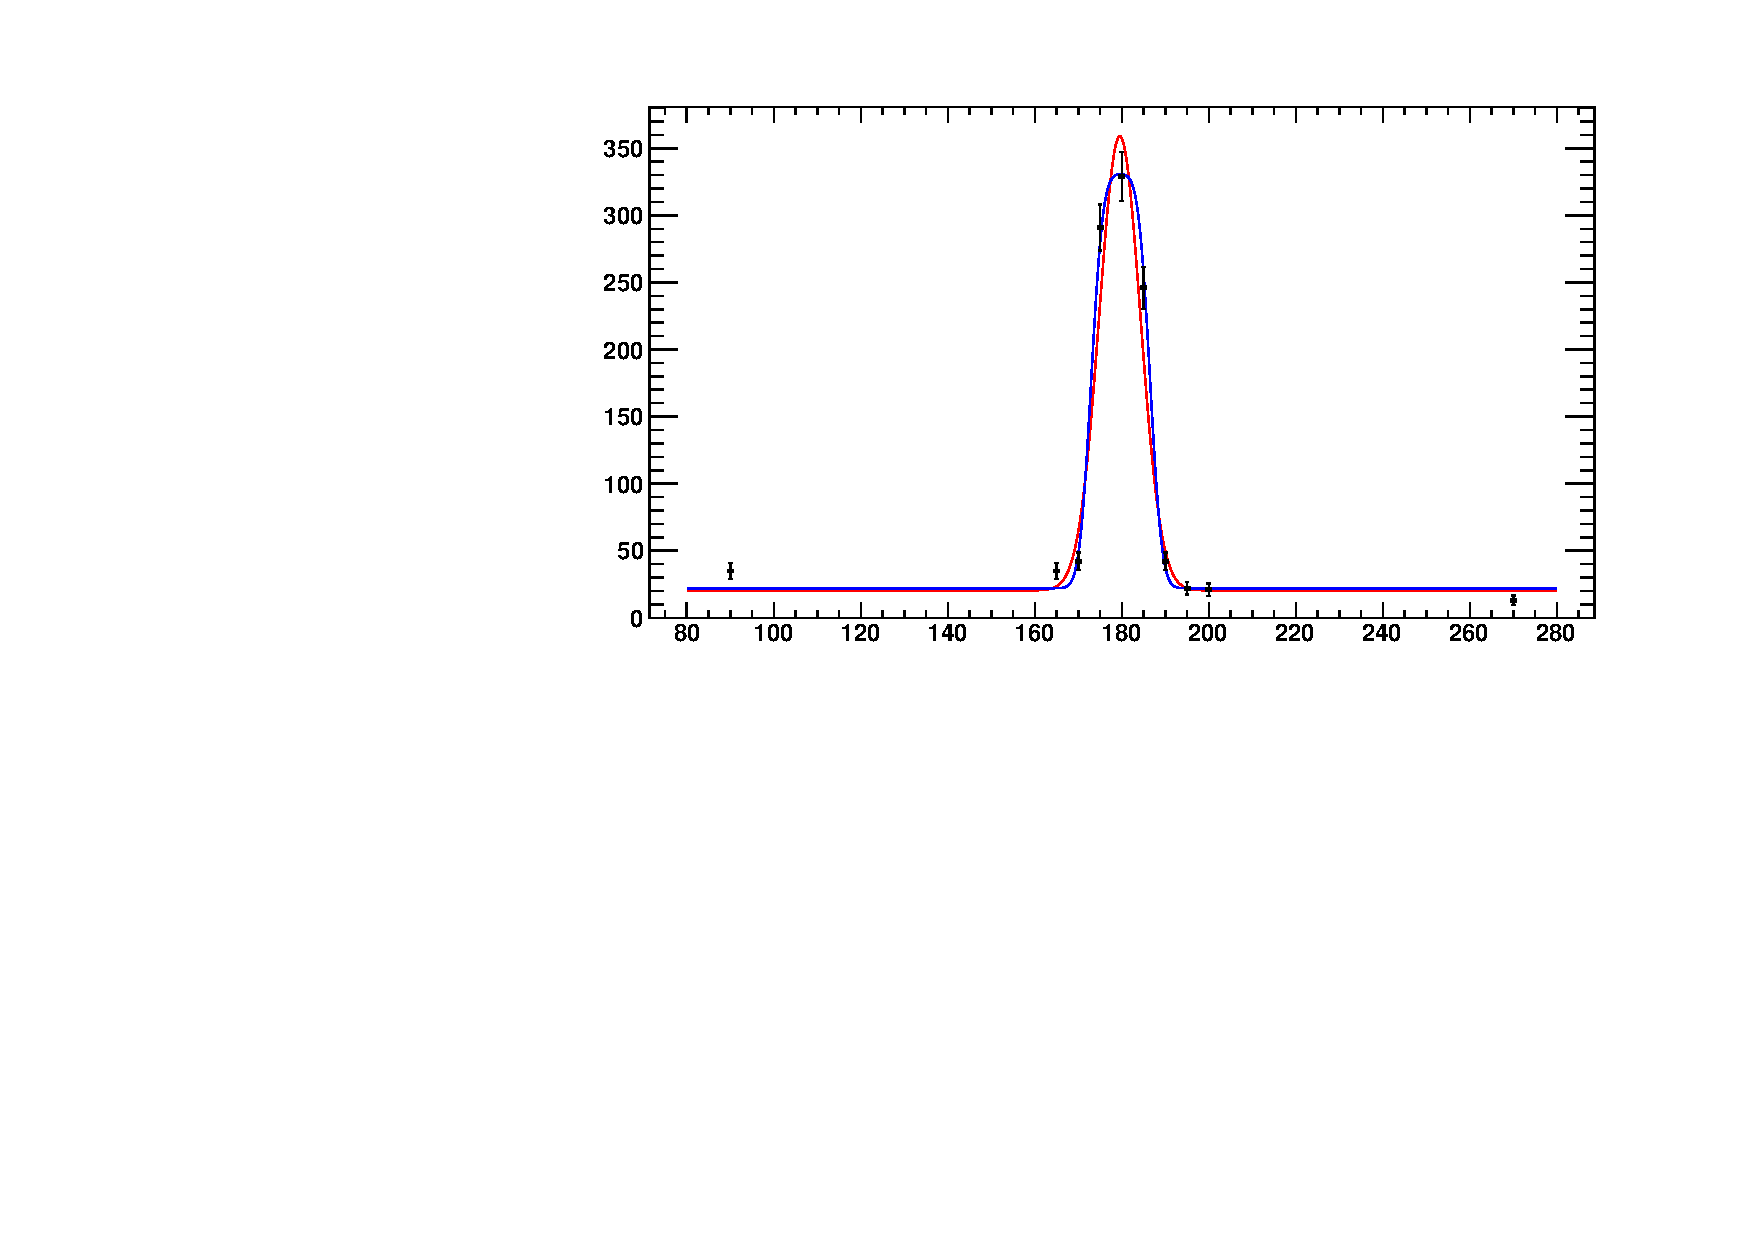
\includegraphics[width=\textwidth]{../img/angles.pdf}
  \caption{Winkelkorrelation der \na-Vernichtungsphotonen.
  Modellierung mit Gaußverteilung (rot) und
  mit Faltung von Rechtecksfunktion und Gaußkurve (blau), beide auf linearem Untergrund.}
  \label{img:angles}
\end{center}
\end{figure}

\autoref{img:angles} zeigt die Winkelabhängkeit der Zählereignisse bei der Messung an \na.
Für die Berechnung des Fehlers wurde gemäß der Poissonverteilung \autoref{eq:poisson:error} verwendet.
Deutlich sichtbar ist die Häufung der Zählereignisse um den Winkelbereich bei 180$^\circ$.
Dieser Bereich wurde zuerst mit einer Gaußfunktion modelliert,
der Untergrund mit der Addition einer konstanten Funktion $a$.
Die Parameter des Fits befinden sich auf \autoref{tab:angfit}.
Da allerdings von den fünf höchsten Messwerten keiner die Fitfunktion innerhalb seiner Fehlergrenzen einschließt,
wurde nach einem besseren Modell gesucht.\\
Der Messaufbau legt nahe, eine Rechtecksfunktion $R$ mit Breite $b$ zur Modellierung zu verwenden,
da der NaI-Szintillationszähler einen relativ großen Öffnungswinkel besitzt,
innerhalb dessen Photonen registriert werden können:
\begin{equation}
  R(x;b) =
\begin{cases}
1 & \text{für }\frac{-b}{2} \leq x \leq \frac{b}{2}\\
0 & \text{sonst}
\end{cases}
\end{equation}
Fallen die Photonen allerdings auf den Rand des Szintillators,
so nimmt die Wahrscheinlichkeit ab, dass genügend Sekundärphotonen erzeugt werden,
um einen Zählpuls auszulösen.
Diese Überlegung führt dazu, dass als Modell für die Anzahl der Zählereignisse~$N$ in Abhängigkeit des Winkels~$x$
das \emph{Faltungsprodukt} einer Rechtecksfunktion mit einer
Gaußfunktion verwendet wird:
\begin{equation}
\begin{split}
  N(x;b,A,\alpha_0,s)&=R(x;b)*\gaus(x;A,\alpha_0,s)\\
  & = \int_{-\infty}^{\infty}{R(\tau;b) \cdot  \gaus(x-\tau;A,\alpha_0,s) \, \difd\tau}\\
  & =   \frac{A}{2} \left(\text{erf}\left(\frac{b+2 \alpha_0 -2 x}{\sqrt{8} s }\right)+
  \text{erf}\left(\frac{b-2 \alpha_0 +2 x}{\sqrt{8} s }\right)\right)
\end{split}
\end{equation}
Die Funktion erf ist hier die Gaußsche Fehlerfunktion.
Die Werte für die vier Parameter der Fitfunktion und für den linearen Untergrund sind ebenfalls
in \autoref{tab:angfit} aufgeführt.

\begin{table}[H]
\caption{Fitparameter für die Messung der Winkelkorrelation.}
\begin{center}
\begin{tabular}{|c|c|c|c|c|c|c|}
  \hline
   & $\chi^2 / \text{DoF}$ & $b$ & $A$ & $\alpha_0$ & $s$ & $a$ \\ \hline  
 Gaußkurve  & 4.9 & - & 339 $\pm$ 16 & 179.5 $\pm$ 0.4 & 4.7 $\pm$ 0.3 & 20 $\pm$ 2 \\ \hline  
 Faltungsprodukt & 3.3 & 13.6 $\pm$ 0.9 & 309 $\pm$ 18  & 179.7 $\pm$ 0.3 & 2.1 $\pm$ 0.3 & 22 $\pm$ 2 \\ \hline 
 
\end{tabular}
\end{center}
\label{tab:angfit}
\end{table}

Der niedrigere, auf die Zahl der Freiheitsgrade normierte Wert für $\chi^2$ des Fits für das zweite Modell
gibt einen Hinweis darauf, dass dieses Modell besser für die Beschreibung der Daten geeignet ist.
Um das aber eindeutig zu zeigen, wären mehr Messungen um das Intensitätsmaximum notwendig gewesen.\\
Warum der Untergrund nicht gut durch eine lineare Funktion beschrieben werden kann,
konnte nicht geklärt werden.
Für die Entscheidung, ob es sich hier um eine statistische Schwankung oder eine wirkliche
Inhomogenität des Untergrunds handelt, wären ebenfalls mehr Messungen notwendig gewesen.\\
Beide Fits liefern aber eine enge Verteilung der Strahlungsintensität um das Maximum bei 180$^\circ$
und eine Breite der Verteilung, die mit den geometrischen Gegebenheiten des Aufbaus in Verbindung gebracht
werden kann.
Mit dem Experiment konnte also gezeigt werden, dass bei der Annihilation eines Positron-Elektron-Paars
zwei \textgamma-Photonen in entgegengesetzte Richtung emittiert werden.


